\documentclass[12pt,onecolumn,conference]{IEEEtran}

% ---------------------------------------------------------------------------
% Language and fonts
% ---------------------------------------------------------------------------
\usepackage[utf8]{inputenc}
\usepackage[T1]{fontenc}
\usepackage[english]{babel}

% ---------------------------------------------------------------------------
% Page geometry
% ---------------------------------------------------------------------------
\usepackage[margin=2.5cm]{geometry}

% ---------------------------------------------------------------------------
% Units and quantities
% ---------------------------------------------------------------------------
\usepackage{siunitx}
\sisetup{per-mode=symbol}
\DeclareSIUnit\byte{B}
\DeclareSIUnit\GHz{\giga\hertz}
\DeclareSIUnit\dBm{dBm}

% ---------------------------------------------------------------------------
% Graphics and figures
% ---------------------------------------------------------------------------
\usepackage{graphicx}
\graphicspath{{figures/}}
\usepackage{caption}
\usepackage{float}
\usepackage{placeins}
% Stack floats at the top of float-only pages instead of spreading them vertically
\makeatletter
\setlength{\@fptop}{0pt}
\setlength{\@fpsep}{12pt plus 2pt}
\setlength{\@fpbot}{0pt plus 1fil}
\makeatother
\usepackage{booktabs}
\usepackage{array}
\usepackage{tabularx}
\renewcommand{\tabularxcolumn}[1]{m{#1}}

% ---------------------------------------------------------------------------
% Code listings
% ---------------------------------------------------------------------------
\usepackage[dvipsnames]{xcolor}
\usepackage{listings}
\lstdefinestyle{codestyle}{
    basicstyle=\ttfamily\small,
    keywordstyle=\color{blue},
    commentstyle=\color{OliveGreen},
    stringstyle=\color{purple},
    numbers=left,
    numberstyle=\tiny\color{gray},
    stepnumber=1,
    numbersep=8pt,
    backgroundcolor=\color{black!3},
    frame=single,
    breaklines=true,
    breakatwhitespace=false,
    showstringspaces=false,
    tabsize=4
}
\lstset{style=codestyle}

% ---------------------------------------------------------------------------
% Hyperlinks and cross-referencing
% ---------------------------------------------------------------------------
\usepackage[hidelinks]{hyperref}

% ---------------------------------------------------------------------------
% Page style: centered page numbers, running header
% ---------------------------------------------------------------------------
\usepackage{fancyhdr}
\pagestyle{fancy}
\fancyhf{}
\fancyhead[L]{Channel History for Single-BS 5G Localization}
\fancyhead[R]{Battat et al.}
\fancyfoot[C]{\thepage}
\renewcommand{\headrulewidth}{0.4pt}
\renewcommand{\footrulewidth}{0pt}

\fancypagestyle{titlepage}{
  \fancyhf{}
  \fancyfoot[C]{\thepage}
  \renewcommand{\headrulewidth}{0pt}
}

% ---------------------------------------------------------------------------
% Section heading styling
% ---------------------------------------------------------------------------
\usepackage{titlesec}
\titleformat{\subsection}
  {\normalfont\normalsize\bfseries\itshape}
  {\thesubsectiondis}
  {0.5em}
  {}
\titlespacing*{\subsection}{0pt}{1.5ex plus 1.5ex minus 0.5ex}{0.7ex plus .5ex minus 0ex}
\titleformat{\subsubsection}
  {\normalfont\normalsize\bfseries}
  {}
  {0pt}
  {}
\titlespacing*{\subsubsection}{0pt}{1.5ex plus 1.5ex minus 0.5ex}{0.7ex plus .5ex minus 0ex}

% ---------------------------------------------------------------------------
% Miscellaneous
% ---------------------------------------------------------------------------
\usepackage{enumitem}
\usepackage{amsmath}
\usepackage{amssymb}

% ---------------------------------------------------------------------------
% Review/annotation commands
% ---------------------------------------------------------------------------
\newcommand\asl[1]{{\bf\color{red}$<$ASL: #1$>$}}
\newcommand\uncertain[1]{{\color{orange}#1}}
% Every \asl{} and \pending{} is listed in REVIEW_ITEMS.md; remove each once resolved.
\newcommand\pending[1]{{\color{magenta}#1}}

% ---------------------------------------------------------------------------
% Title page metadata
% ---------------------------------------------------------------------------
\title{Using Channel History to Improve\\UE Localization Accuracy in\\Single-Base-Station 5G Networks}
\author{
  \IEEEauthorblockN{Gilad Battat\IEEEauthorrefmark{1},
                    Alon S.~Levin\IEEEauthorrefmark{2},
                    David Sarne\IEEEauthorrefmark{1},
                    Sarit Kraus\IEEEauthorrefmark{1}}
  \IEEEauthorblockA{\IEEEauthorrefmark{1}Department of Computer Science, Bar-Ilan University}
  \IEEEauthorblockA{\IEEEauthorrefmark{2}Department of Electrical Engineering, Columbia University}
}
\date{October 2026}

\begin{document}

\maketitle
\thispagestyle{titlepage}

\begin{center}
\textit{Technical Report prepared for the IISAC Consortium}\\
\textit{Industry Partners: CEVA, Cellcom}
\end{center}

% No abstract in the technical report; the source file is kept.
% \newpage
% \begin{abstract}
% DRAFT for author review. Every number is from the results of record; see docs/paper/REPORT_SKELETON_VALIDATION.md.
A single serving base station fixes a device's range from received signal strength but not its bearing. We ask whether a short window of past measurements, the transition history, narrows this distance-ring ambiguity, in a simulated 5G NR deployment that compares a small controlled grid with a $96\,\text{m}$ macro cell, and across seven estimators from $k$-nearest neighbors to recurrent, convolutional and attention networks.
For devices that report an angle of arrival, five steps of history ($20\,\text{m}$ of travel) lower the position error by $2.8$ to $4.1\,\text{m}$ ($15$ to $21\%$) in all seven families, and model choice barely matters.
In the macro cell the gain comes entirely from the angle channels, and it is the averaging of imperfect angle reports: an unordered mean of the window reproduces it, elevation carries most of it, and with exact angles it disappears. It therefore depends on the angle error being independent between reports, falling from about $17\%$ to $2$ to $6\%$ when the error persists.
Devices without an angle gain no more than about $1\%$ on uniform non-line-of-sight propagation, where their models beat a constant guess of the cell centre by only $5$ to $6\%$; with mixed LOS and NLOS propagation, tree ensembles gain about $1.2\,\text{m}$, an effect linked to the propagation state.
Line-of-sight propagation, interfering base stations and a blocked line of sight do not change the multi-antenna gain. On the controlled grid, history raises accuracy under all three propagation settings tested, with and without an angle; there a recurrent network and a convolutional network keep improving up to fifteen steps while tree ensembles stop at about three, and shuffling the older reports inside the window, with the current report kept in place, raises the recurrent network's error at fifteen steps by $19$ to $48\%$, so on the grid the order of the reports carries information beyond their mean.
\end{abstract}


\newpage \tableofcontents

\newpage
\section{Introduction}
\label{sec:introduction}

% src: 47 CFR 9.10(i)(2)(i) (dispatchable location or x/y within 50 m for 80 % of wireless 911 calls within 6 years; law.cornell.edu, verified 2026-10-30); Italiano et al. 2025 p. 5 (emergency-call requirements drove cellular localization; "support emergency services and foster location-based applications"; asset tracking), p. 2 (5G "complementing GNSS ... in outdoor positioning and navigation"); Groves 2011 abstract ("GPS is unreliable in dense urban areas ... buildings block the signals from many of the satellites")
Locating a user equipment~(UE) from the cellular network is a regulatory requirement and an enabler of location-based services. In the United States, wireless carriers must locate \SI{80}{\percent} of wireless 911 calls to within \SI{50}{\meter}~\cite{cfr47_9_10}, and cellular positioning also serves applications such as asset tracking and navigation~\cite{italiano2025tutorial}. The need is sharpest where satellite positioning is weakest, as in dense urban areas, where buildings block the signals of many satellites~\cite{groves2011shadow}.

% src: 3GPP TS 38.215 §5.1 (UE: SS-RSRP, SS-SINR), §5.2 (gNB: UL AoA, TADV); TS 38.305 §4.3.10 (NR E-CID: "the UE generally is not expected to make additional measurements for the sole purpose of positioning"), §8.9.1 (E-CID inputs); verified on itecspec.com 2026-10-30
The cellular network is well placed to meet this need, because it already observes every connected UE. In 5G New Radio~(NR), the UE measures and reports its signal-to-interference-plus-noise ratio~(SINR) and its received signal strength~(RSS), reported as the reference signal received power~(RSRP), while the base station~(BS) measures the uplink angle of arrival~(AoA) and the timing advance~\cite{3gpp38215}. The standardized enhanced cell-ID method uses these measurements for positioning without requiring any made for that purpose alone~\cite{3gpp38305}, so the network can position a UE without an added receiver, sensor or infrastructure.

% src: Italiano et al. 2025 p. 14 (RSS path-loss model Eqs. (14)-(15); power-based measurements are "reasonable distance indicators only if the BS is near to the UE", shadowing and multipath), p. 22 ("DL-TDOA requires precise synchronization among the BSs"; RTT does not)
The difficulty is accuracy. RSS depends mainly on the distance to the BS and is perturbed by shadowing and multipath, so it is a reasonable distance indicator only near the BS~\cite{italiano2025tutorial}, and it carries no information on the bearing. Geometric positioning recovers the bearing by combining time or angle measurements from several BSs, and its time-difference methods further require precise synchronization among them~\cite{italiano2025tutorial}. A single serving BS, however, provides at most one range and, where an angle is available, one bearing; without a reliable angle, a single report leaves the position under-determined. This case would benefit most from a solution that adds no infrastructure. We address it by using the history of a UE's reports, not only the current one.

\subsection{The Channel History Hypothesis}
\label{subsec:ambiguity-hypothesis}

% src: FINAL_REPORT.md §1.1, §1.2, §3.2
The hypothesis evaluated in this work is that a moving UE's sequence of reports carries more positional information than any single report, and that this holds regardless of the estimator applied on top of it. Because the radio channel is spatially consistent, consecutive reports of a moving UE are correlated samples of the channel along its path, and a window of them shows how the measurements change as the UE moves, which no single report contains.

The ambiguity of a single report is one reason to expect such a gain. RSS depends mainly on the distance to the BS, so a single reading constrains the range, up to shadow fading, but not the bearing: positions on a common range ring around the BS are indistinguishable to a single-snapshot estimator, which we refer to as the \emph{distance-ring ambiguity}. SINR and AoA can each supply bearing information, but both are conditional, since SINR depends on the placement of interfering BSs and AoA on UE hardware that legacy single-antenna devices lack. Two positions on the same ring, however, produce different sequences of reports, because the channel around each evolves differently as the UE moves. A history of reports may therefore resolve what a single report cannot, without additional infrastructure; this work tests whether it does so across propagation settings, BS placements and estimators.

\subsection{Contributions}
\label{subsec:contributions}

% src: CLAIM_EVIDENCE_MAP.md (2026-10-24) core message and C1-C9; studies G, R, M as defined there
We evaluate this hypothesis in three simulated studies of a single 5G NR BS: a controlled $15\times15$ grid on which the exact cell is classified, $25\times25$ regression runs that pool five device profiles, and a macro cell in which every model is tested on users not seen in training. Using the history of a user's reports, rather than the current report alone, consistently lowers the error of the best model across propagation settings, BS placements and model families. The gain depends on the position information a single report carries and on whether that information is shared between users: where one report carries nothing that transfers to new users, as for single-antenna devices in the uniform-NLOS macro cell, whose users are each simulated as a separate channel realization, history adds nothing, whereas in a simulated environment shared by all users, history lowers the error of unseen users, under uniform NLOS as well.

Specifically, the contributions of this work are the following: (i) a consistent history gain, measured for the best model in every propagation setting and BS placement of the three studies and in all seven model families of the macro cell, and robust to propagation, blockage and interference, thereby making the input, rather than the estimator, the deciding design choice; (ii) evidence that sequence models exploit long windows where tree ensembles given the same window cannot, together with a test showing that the order of the reports carries part of that gain on the grid; (iii) an account of the macro-cell gain as the averaging of noisy angle reports, and of how it shrinks when the angle error persists across reports; and (iv) a delimitation of where history adds nothing, namely where a single report carries no position information that transfers between users, together with a test showing that this depends largely on the simulation: when all users share one simulated environment, history lowers the error of unseen users, also under uniform NLOS, and differences between consecutive reports become informative.

\noindent\textbf{Organization.} Section~\ref{sec:related-work} reviews related work. Section~\ref{sec:system-model} formulates the problem and what history can add to a single report. Section~\ref{sec:setup} describes the simulated deployments, devices, features, estimators and evaluation protocol. Section~\ref{sec:results-gain} presents the history gain across the three studies and its robustness to propagation, blockage and interference; Section~\ref{sec:results-window} then compares how tree ensembles, sequence models and a tracking filter use the window, and Section~\ref{sec:results-mechanism} identifies what history reads in the macro cell. Section~\ref{sec:results-no-gain} examines the one setting in which history adds nothing. Section~\ref{sec:discussion} discusses the results and their limitations; Section~\ref{sec:conclusion} concludes.


\subsection{Related Work}
\label{sec:related-work}

% src: FINAL_REPORT.md §2, "Fingerprinting" paragraph
Classical RSS fingerprinting matches a measurement snapshot against a surveyed database~\cite{yang2013_rssitocsi}; single-site multipath fingerprinting establishes that one BS already observes enough structure to localize without triangulation~\cite{kupershtein2013}, the principle this work extends to a moving user. Fingerprinting's characteristic failure mode is poor discrimination between points at equal range from the BS, which is exactly the distance-ring ambiguity a history of reports targets.
The static $k$-nearest-neighbor~($k$-NN) regressor at $h=0$ represents this family throughout this work. % src: FINAL_REPORT.md §2 (k-NN h=0 baseline)

% src: FINAL_REPORT.md §2, "Geometric methods" paragraph
Geometric methods recover position from an explicit system built on time-of-arrival, time-difference-of-arrival, or AoA estimates~\cite{italiano2025tutorial}.
These methods require either multiple synchronized BSs or a high-quality angle estimate, so the single-serving-BS, single-angle-source deployment studied here is precisely the regime in which the geometric system is underdetermined: for a device that reports no angle at all, the available geometry constrains range but leaves bearing unresolved anywhere along the range ring.

% src: FINAL_REPORT.md §2, "Sequence models for CSI" paragraph
Recurrent and dynamic-system formulations have likewise been applied to channel state information~(CSI)-based tracking~\cite{fang2010dynamic,yu2020rnn,shi2018tracking}, and a related line shows that the temporal autocorrelation of RSS improves fingerprinting accuracy when the signal is treated as a stationary process observed at a fixed location~\cite{wang2016temporal,tian2018temporal}. That signal differs from the one used here: it is order-invariant and aggregated across access points, so it survives for a stationary receiver and vanishes for a moving one, whereas the channel-history window used here is ordered, is read from a single BS, and encodes exactly the motion the in-place statistic discards. These works propose a tracking architecture and evaluate it as a whole, so the benefit of the temporal input cannot be separated from that of the architecture. In this work, we instead hold each estimator fixed and vary only the history window it receives, thereby isolating the contribution of history, and repeat the comparison across model families.

\section{System Model and Problem Formulation}
\label{sec:system-model}

In this section, we define the measurements a serving BS observes, set out what a window of them can add to a single report, and state the two estimation tasks.

\subsection{Measurement Model}
\label{subsec:measurement-model}

% src: FINAL_REPORT.md §3.1
At discrete snapshot time~$t$ the serving BS observes the measurement vector
\begin{equation}
  \mathbf{m}(t) = \big[\, \mathrm{RSS}(t),\ \mathrm{SINR}(t),\ \theta_{az}(t),\ \theta_{el}(t) \,\big],
  \label{eq:measurement-vector}
\end{equation}
with the azimuth/elevation pair $(\theta_{az}, \theta_{el})$ present only for UEs whose antenna count $N_{ant} \ge 2$, i.e. \emph{multi-antenna devices}, as opposed to \emph{single-antenna devices}. The channel experienced by multi-antenna UEs is modeled by maximum-ratio combining over the per-element channel,
\begin{equation}
  H_{\text{eff}}(f) = \sqrt{\textstyle\sum_{i=1}^{N_{ant}} \lvert H_i(f) \rvert^2},
  \label{eq:mrc}
\end{equation}
with a device-specific antenna-gain offset applied additively in dB.

% src: FINAL_REPORT.md §3.3 (window definition)
Given a history depth~$h$, the model input is the window of $h+1$ consecutive measurement vectors,
\begin{equation}
  \mathcal{W}_h(t) = \left[\, \mathbf{m}(t-h),\ \dots,\ \mathbf{m}(t) \,\right],
  \label{eq:transition-history}
\end{equation}
where $h=0$ is the single-report input. %UEs with $N_{ant} \ge 2$ are called multi-antenna devices, and those with $N_{ant} = 1$ single-antenna devices.

\subsection{What History Can Add}
\label{subsec:history-dof}
% src: FINAL_REPORT.md §1.1, §3.2; model: Italiano et al. 2025 Eqs. (14)-(15) (p. 14); TR 38.901 §7.4.1 (log-distance PL, log-normal shadow fading sigma_SF; itecspec.com, verified 2026-10-30)
Let $\mathbf{p}_{UE}$ and $\mathbf{p}_{BS}$ denote the UE and serving-BS positions, and let $r = \lVert \mathbf{p}_{UE} - \mathbf{p}_{BS} \rVert$ be their range. Under the log-distance path-loss model with log-normal shadow fading~\cite{italiano2025tutorial,3gpp38901},
\begin{equation}
  \mathrm{RSS} \approx P_{tx} - 10\gamma\log_{10} r + \chi,
  \label{eq:path-loss}
\end{equation}
where $P_{tx}$ is the transmit power, $\gamma$ the path-loss exponent and $\chi$ zero-mean shadow fading of standard deviation~$\sigma$. A single RSS value therefore identifies $r$ up to $\chi$ but leaves the bearing unconstrained, which is the distance-ring ambiguity of Section~\ref{subsec:ambiguity-hypothesis}.

A window can add to a single report in two distinct ways, which make different predictions and are tested separately in this work.

% src: FINAL_REPORT.md §3.3; csi_dataset.py build_derived_features (first differences of RSS, azimuth and ray coordinates divided by delta_t)
\noindent\textbf{Rates of change.} Consecutive reports of one UE, a time $\Delta t$ apart, give finite differences such as $[\mathrm{RSS}(t)-\mathrm{RSS}(t-1)]/\Delta t$, which approximate the time derivatives of the measurements; a window of depth $h$ gives $h$ such differences and therefore also their evolution. The raw window contains the consecutive values from which these differences follow, and the macro-cell features also supply the first differences of RSS, azimuth and the two ray coordinates explicitly~(Section~\ref{subsec:features}). Two of the derivatives carry geometric meaning. The rate of change of RSS,
\begin{equation}
  \frac{d\,\mathrm{RSS}}{dt} \approx -\frac{10\gamma}{\ln 10} \cdot \frac{\dot r}{r},
  \label{eq:drss-dt}
\end{equation}
reflects the radial component of the motion, and, where AoA is available, the angular rate,
\begin{equation}
  \dot\theta_{az} = \frac{v_\perp}{r},
  \label{eq:dtheta-dt}
\end{equation}
gives the tangential component $v_\perp$ of the velocity and, jointly with $\dot r$, the heading.

% src: FINAL_REPORT.md §7.5 (dRSS/dr expression); Equation (path-loss) above
Without AoA, only the first of these is available, and its usefulness is bounded by the path-loss gradient. Differentiating Equation~(\ref{eq:path-loss}) with respect to range gives
\begin{equation}
  \left\lvert \frac{d\,\mathrm{RSS}}{dr} \right\rvert = \frac{10\gamma}{r \ln 10}\ \text{dB/m},
  \label{eq:rss-gradient}
\end{equation}
so a step of fixed length moves RSS by an amount that falls as $1/r$, while the shadow-fading spread $\sigma$ does not shrink with range. RSS differences are therefore expected to carry less information far from the BS; Section~\ref{sec:results-no-gain} tests this expectation. Because a difference depends on which report precedes which, this mechanism requires the order of the reports.

% src: FINAL_REPORT.md §3.3; technical_documentation_revised.md 6.5 (averaging account of the angle history)
\noindent\textbf{Repeated noisy samples.} Over a short window the UE moves little compared with its range, so the reports are also several noisy samples of nearly the same quantities. Averaging them reduces the measurement error, such as the AoA estimation noise and quantization, independently of any information about the motion. This mechanism requires neither the order of the reports nor any motion, and it adds nothing when the measurements are exact.

The two mechanisms are therefore distinguished by whether the order of the reports matters, whether an unordered mean of the window recovers the gain, and whether the gain survives exact measurements; Sections~\ref{sec:results-window} and~\ref{sec:results-mechanism} apply these tests.

\subsection{Task Formulations}
\label{subsec:task-formulations}

% src: FINAL_REPORT.md §3.4; technical_documentation.md §7.4 (625-class memory limit)
We evaluate two task formulations. \emph{Classification} predicts one of $G$ discrete grid cells and is appropriate when the grid spacing greatly exceeds the position jitter. \emph{Regression} predicts a continuous position relative to the serving BS and is scored by the 2D Euclidean error. In the two larger deployments, UEs still move between the points of a $25\times25$ grid, but a classifier over its $625$ points is memory-prohibitive, so position is estimated by regression instead.

\section{Experimental Setup}
\label{sec:setup}

In this section, we describe how the data were generated and evaluated. Section~\ref{subsec:channel-simulation} describes the channel simulation; Sections~\ref{subsec:studies}--\ref{subsec:device-model} describe the deployments, the mobility and the devices, and Sections~\ref{subsec:features}--\ref{subsec:protocol} the features, estimators and evaluation protocol.

\subsection{Channel Simulation}
\label{subsec:channel-simulation}

% src: FINAL_REPORT.md §4.2; configs (*_15x15, *_25x25: bandwidth 1e8)
All data are generated with QuaDRiGa, a 3GPP TR~38.901-compliant channel simulator~\cite{3gpp38901,quadriga_paper,quadriga_website}, at \SI{3.0}{\giga\hertz} center frequency with \SI{100}{\mega\hertz} bandwidth, with $256$ orthogonal frequency-division multiplexing~(OFDM) subcarriers, \SI{30}{\dBm} transmit power per site, and an omnidirectional BS antenna element. This work extends a time-aware multi-user massive multiple-input multiple-output~(MIMO) simulator developed within the same research group~\cite{Israeli_5G_Massive_MIMO_2026,israeli_sarne_simulation}, to which we added grid-constrained trajectory generation and the device-heterogeneity model that is described in Section~\ref{subsec:device-model}.

% src: FINAL_REPORT.md §4.2 ("What interference means here")
Where a deployment includes interfering BSs in addition to the serving BS, SINR is computed as
\begin{equation}
  \mathrm{SINR} = \frac{P_{\text{serving}}}{\sum_i P_{\text{IBS-}i} + P_{\text{noise}}},
  \label{eq:sinr}
\end{equation}
where $P_{\text{serving}}$ and $P_{\text{IBS-}i}$ are the received powers from the serving BS and the $i$-th interfering BS, and $P_{\text{noise}} = \SI{-104}{\dBm}$ is the noise power, a fixed setting of the simulation. Interference is therefore contributed only by the modeled interfering sites; no user-to-user coupling is represented, and a user's SINR does not depend on how many other users are simulated.

\subsection{Studies}
\label{subsec:studies}

% src: FINAL_REPORT.md §4.1, §7.5 ("eight differences"); technical_documentation.md §3, §7.1, §7.3.3, §7.4; configs/multi_user_voronoi_15x15_config.jsonc, ne_bs_voronoi_15x15_config.jsonc, ne_bs_voronoi_25x25_config.jsonc (center_frequency, grid, base_station)
We draw the evidence from three simulated deployments at two scales, summarized in Table~\ref{tab:studies}. The \emph{controlled-grid study} places UEs on a $15\times15$ grid at \SI{2}{\meter} pitch within \SI{20}{\meter} of the serving BS and predicts the exact cell, under conditions chosen to be clean and repeatable. The \emph{macro-cell study} places $300$ users on a $25\times25$ grid at \SI{4}{\meter} pitch, $21$ to \SI{157}{\meter} from an off-grid serving BS, predicts continuous position, and evaluates on users never seen during training. The \emph{$25\times25$ regression runs} share the macro-cell geometry but, like the controlled grid, split each user's walk in time; they simulate five device profiles, one user each, pooled in one model, under three propagation settings: urban-micro~(UMi) line-of-sight~(LOS), uniform UMi non-line-of-sight~(NLOS), and a per-cell mix of the two. As a design choice, the reference history depth is $h=3$ in the controlled-grid study and the $25\times25$ runs and $h=5$ in the macro-cell study; the sequence models of the first two are evaluated up to $h=15$, and other depths are stated where used. A fourth deployment, a corridor with a blocked line of sight, is described in Section~\ref{subsec:robustness}.

\begin{table}[t]
  \centering
  \caption{The three simulated deployments.}
  \label{tab:studies}
  \small
  \begin{tabularx}{\textwidth}{@{}lXXX@{}}
    \toprule
     & Controlled-grid study & $25\times25$ regression runs & Macro-cell study \\
    \midrule
    Task & Classification~(225 cells) & Regression & Regression \\
    Grid, pitch & $15\times15$, \SI{2}{\meter} & $25\times25$, \SI{4}{\meter} & $25\times25$, \SI{4}{\meter} \\
    Service area & \qtyproduct{28 x 28}{\meter} & \qtyproduct{96 x 96}{\meter} & \qtyproduct{96 x 96}{\meter} \\
    Range to serving BS & $0$--\SI{20}{\meter}~(center BS); $21$--\SI{61}{\meter}~(corner BS) & $21$--\SI{157}{\meter} & $21$--\SI{157}{\meter}, mean \SI{93}{\meter} \\
    Serving BS~(m) & $[19,19,10]$~(center) or $[48,48,10]$~(corner) & $[116,116,10]$ & $[116,116,10]$ \\
    Carrier & \SI{3.0}{\giga\hertz} & \SI{3.0}{\giga\hertz} & \SI{3.0}{\giga\hertz} \\
    Population & 5 device profiles, $450{,}005$ samples & 5 device profiles, one user each, $1{,}250{,}000$ samples, \SI{30}{\percent} of training samples used & 300 users simulated, 232 retained, 47 tested per split \\
    Split & Chronological $80/20$ within each user & Chronological, or shuffled 5-step blocks & $80/20$ over disjoint users \\
    Mobility & Random walk, \SI{1.5}{\meter\per\second} & Random walk & Four patterns, $0.1$--\SI{15}{\meter\per\second} \\
    AoA impairment & SINR-dependent noise, \ang{5} quantization & \ang{4} Gaussian noise, \ang{5} quantization & \ang{4} Gaussian noise, \ang{5} quantization \\
    Repetitions & Single run~(trees); three seeds~(sequence models) & Single run; three seeds for the GRU at $h=15$ & $20$ user splits~(XGBoost, Random Forest); five~(other models) \\
    \bottomrule
  \end{tabularx}
\end{table}
% src (macro-cell AoA impairment): CSI-Location src/python/utils/csi_dataset.py load_and_prepare_data (aoa_noise_std_deg=4.0, aoa_quant_step_deg=5.0); 232 retained: FINAL_REPORT.md §4.3; 47 test users: seed_repeats_all_models_summary.json per-run n_test_users; range 21.2-157.0 m, mean 93.2: FINAL_REPORT.md §7.5

% src: configs/multi_user_voronoi_15x15_config.jsonc (BS [19,19,10]; interferers [-11,19,10], [19,-11,10]); ne_bs_voronoi_15x15_config.jsonc (BS [48,48,10]; same interferers); both read by core/generate_simulation_data.m; technical_documentation.md §7.3 (~52 degree azimuth spread)
% src: results_of_record/controlled_grid_2026_10/comparison_sets.md (RMa LOS, mixed per-cell, uniform NLOS at 3.0 GHz)
In the controlled-grid study the serving BS sits either at the grid center, where the grid spans the full \ang{360} of azimuth, or beyond the north-east corner, where all $225$ cells fall within a wedge of about \ang{52}; two interfering sites enter through Equation~(\ref{eq:sinr}) for both placements. The grid is simulated under three propagation settings: rural-macro~(RMa) LOS for every walk; a mixed setting in which each of four Voronoi zones has its own UMi LOS or NLOS scenario, so that the propagation changes along a walk; and uniform UMi NLOS. Figure~\ref{fig:layout} draws the controlled grid and the macro cell to the same scale.

% src: configs/ne_bs_voronoi_25x25_config.jsonc (BS [116,116,10]); FINAL_REPORT.md §4.1 (interferers); FINAL_REPORT.md §5.6 (uniform NLOS primary); CONTINUE_HERE.md §3 (per-segment mixed runner)
In the macro-cell study the serving BS sits off-grid to the north-east, again with two interfering sites. The primary realization of this study uses a single UMi NLOS propagation profile for every user. A second realization assigns each of four Voronoi regions its own profile, LOS for the park to the north and the highway to the south-west and NLOS for the shopping district to the south-east and the residential area to the south, and generates each scenario segment of a trajectory as an independent channel; it serves to test how propagation conditions change the result.

\begin{figure}[h]
  \centering
  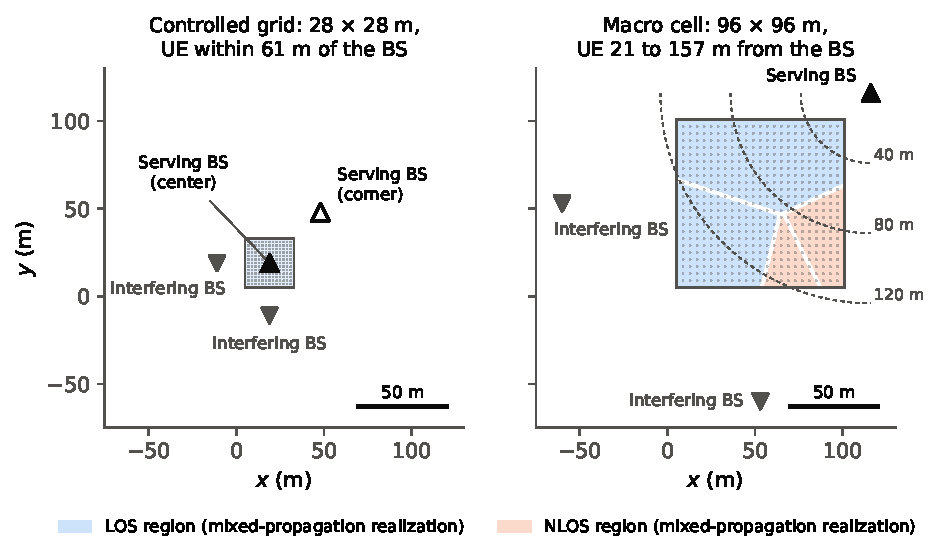
\includegraphics[width=0.95\textwidth]{fig_study_maps}
  \caption{The controlled grid with its two serving-BS placements~(left) and the macro cell with its four Voronoi regions~(right), at the same scale. Filled and open markers give the center and corner placements; arcs give the range from the macro-cell BS.}
  \label{fig:layout}
\end{figure}
% src: figure_scripts/python/make_figures.py study_maps(); grids, BS positions and Voronoi centres from the 15x15 and 25x25 configs; macro-cell transmitters from runners/run_multi_user_300_25x25.m (the 25x25 config's interferer entries, [-25,53] and [53,-25], are not used by that runner)


\subsection{Mobility}
\label{subsec:mobility}

% src: FINAL_REPORT.md §4.3
The controlled-grid study moves each UE on a random walk over the $8$-connected grid graph at \SI{1.5}{\meter\per\second}; the walk carries no persistent heading. In the macro-cell study each user follows one of four trajectory patterns, namely boundary-reflecting straight-line navigation, a persistent random walk, a waypoint tour or a straight transit, at a speed between \SI{0.1}{\meter\per\second}~(near-static) and \SI{15}{\meter\per\second}~(vehicular). All four patterns carry heading persistence, so the mobility of the macro cell favors the use of a history of reports.

% src: FINAL_REPORT.md §4.3, §5.8 (every step advances exactly one grid cell); jitter: generate_simulation_data.m l.238-241 (grid, 25x25 runs); none in run_multi_user_300_25x25*.m (macro)
In all three studies, every step of a walk advances exactly one grid cell, and the time between snapshots is the step length divided by the UE's speed. A fixed history depth is therefore a fixed distance travelled, $h$ grid steps, but not a fixed duration: across the $232$ retained macro-cell users the time between snapshots $\Delta t$ ranges from $0.27$ to \SI{32.5}{\second}, with a median of \SI{2.71}{\second}. In the controlled-grid study and the $25\times25$ runs, a jitter of \SI{+-0.1}{\meter} is added to every snapshot so that no estimator can latch onto repeated coordinates; in the macro-cell study, by contrast, the snapshots lie exactly on the grid points.

\subsection{Device Model and AoA Impairment}
\label{subsec:device-model}

% src: FINAL_REPORT.md §4.4; technical_documentation.md §3.6, §3.7
The controlled-grid study simulates five device profiles: two four-antenna devices that differ only in their walk, a two-antenna device, a one-antenna device, and a two-antenna device carried at \SI{0.9}{\meter} height. The macro-cell study draws from a population of \SI{85}{\percent} multi-antenna devices~(about \SI{45}{\percent} with four antennas and \SI{40}{\percent} with two) and \SI{15}{\percent} single-antenna devices, each with its own antenna gain and carrying height. The split is an assumption of this work.
Antenna count enters the channel through Equation~(\ref{eq:mrc}), and AoA capability is imposed when features are built.

% src (footnote): CLAIM_EVIDENCE_MAP.md C7 (single omni BS; AoA = simulator angle + noise, generate_simulation_data.m)
% src: FINAL_REPORT.md §4.4 (SINR-dependent model, controlled grid); csi_dataset.py load_and_prepare_data (macro cell: aoa_noise_std_deg = 4.0, aoa_quant_step_deg = 5.0, AoA = 0 for single-antenna devices)
Clean simulated arrival angles are degraded before use.\footnote{The serving BS has a single omnidirectional element, so the reported AoA is not estimated from an array response; it is the arrival angle of the simulated channel, degraded as described here.} In the controlled-grid study the noise on each axis depends on SINR,
\begin{equation}
  \sigma_{\text{AoA}}(t) = \operatorname{clamp}\!\left(2.0^\circ \cdot 10^{-\frac{\mathrm{SINR}_{dB}(t)-10}{15}},\ 1.0^\circ,\ 20.0^\circ\right),
  \label{eq:aoa-noise}
\end{equation}
whereas the macro-cell study and the $25\times25$ runs apply a fixed Gaussian error of standard deviation $\sigma_{\text{AoA}} = \ang{4}$, drawn independently for every report. Both then quantize azimuth and elevation to a codebook of step $\Delta_{\text{q}} = \ang{5}$. Both impairment models are fixed settings of the simulation pipeline, and Section~\ref{subsec:averaging} varies them. Single-antenna devices cannot form a beam and report no angle; in the macro-cell features their angle is set to \ang{0}.

\subsection{Features}
\label{subsec:features}

% src: technical_documentation.md §4.1-4.3
In the controlled-grid study, $\mathbf{m}(t)$ contains RSS and SINR, optionally extended with the AoA pair and with three device parameters: antenna count, antenna gain, and carrying height. The window of Equation~(\ref{eq:transition-history}) is built per user after sorting by time; the first $h$ snapshots of each user are dropped, and no window crosses from one user to another. Values are stacked in absolute form, because device-specific RSS and SINR offsets are stable and act as fingerprints.

% src: FINAL_REPORT.md §4.5; csi_dataset.py build_derived_features (d_rss, d_az, d_ray_x, d_ray_y are per-user first differences divided by delta_t; ray = FSPL range estimate x AoA unit vector)
In the macro-cell study, each snapshot carries $13$ channels, all computable from the raw measurements: RSS; SINR; the sines and cosines of both angles; two ray-projection coordinates formed from a path-loss range estimate and the AoA unit vector; the time increment $\Delta t$; and the first differences of RSS, azimuth and the two ray coordinates, each divided by $\Delta t$. It should be noted that, because the first differences are part of each snapshot, the $h=0$ input of the macro-cell study already contains one step of change, and the $h=5$ input stacks six such snapshots. Three static device features, namely antenna count, gain and height, accompany every input.

\subsection{Estimators}
\label{subsec:estimators}

% src: CSI-Location experiments_ablation/model_zoo.py (build_classical, build_net, training constants); master_benchmark_rerun_summary.json (n_params)
The macro-cell study evaluates seven estimators spanning five algorithmic paradigms, listed in Table~\ref{tab:estimators}: $k$-NN, Random Forest, XGBoost, a gated recurrent unit~(GRU) network, and three one-dimensional convolutional neural networks~(1D-CNN), one with an AoA-validity channel and one with temporal self-attention. We hold the hyperparameters fixed across history depths, so that the input window is the only factor that varies within a model; their values are given in Appendix~\ref{app:hyperparameters}. The controlled-grid study uses Random Forest and XGBoost classifiers together with a 1D-CNN and a GRU, and the $25\times25$ runs use Random Forest and XGBoost regressors together with the same two sequence models.

\begin{table}[h]
  \centering
  \caption{Estimators used in the macro-cell study.}
  \label{tab:estimators}
  \small
  \begin{tabular}{@{}lll@{}}
    \toprule
    Paradigm & Model & Configuration \\
    \midrule
    Instance-based & $k$-NN & $k=5$ \\
    Bagged trees & Random Forest & 150 trees, depth 16, min.\ leaf 5 \\
    Boosted trees & XGBoost & 50 trees, depth 5, learning rate 0.15 \\
    Recurrent & GRU & 2 layers, 254\,K parameters \\
    Convolutional & 1D-CNN & 3 convolutional layers, 67\,K parameters \\
    Convolutional & Mask-aware 1D-CNN & 1D-CNN with an AoA-validity channel, 67\,K parameters \\
    Attention & 1D-CNN with temporal self-attention & 200\,K parameters \\
    \bottomrule
  \end{tabular}
\end{table}

\subsection{Evaluation Protocol}
\label{subsec:protocol}

% src: FINAL_REPORT.md §4.7; technical_documentation_revised.md 6.2/6.4 (validation block from the training data for the grid and 25x25 sequence models)
The controlled-grid study and the $25\times25$ runs split each user's walk in time, training on the first \SI{80}{\percent} of steps and testing on the last \SI{20}{\percent}; a random split would leak, because spatial consistency makes temporally adjacent samples near-duplicates. The controlled grid is scored by exact-cell accuracy and by the mean distance between the predicted and true cells. The macro-cell study splits over users, so that the $47$ test users of each split are never seen during training, and it is scored by the 2D Euclidean error between predicted and true position. Every macro-cell result is reported separately for multi-antenna and single-antenna devices.

% src: seed_repeats_all_models.py docstring (seed drives split and init; marginal vs seed-paired); followup_2026_10 (20 seeds, XGBoost and RF, Student-t)
The primary comparison is the change in error when history is added, measured within one model against its own $h=0$ input. For the macro-cell results we repeat the whole protocol over $20$ seeds for XGBoost and Random Forest and over five for the other models, each seed drawing a different user split and model initialization. The spread across seeds is dominated by which users land in the test set; the seed-paired difference compares two inputs on the same split and thereby cancels that source, and its \SI{95}{\percent} Student-$t$ confidence interval is reported with each gain.

% src: experiments_ablation/model_zoo.py train_deep docstring (early stopping on test MAE)
The neural models of the macro-cell study select their stopping epoch by error on the test users, whereas those of the controlled grid and the $25\times25$ runs use a validation block taken from the training data. The macro-cell rule applies equally to both depths of a model, so within-model comparisons are unaffected; however, it makes the absolute errors of the neural models, and any comparison between them and the other models, optimistic in their favor.

\section{Results: A Consistent Gain from History}
\label{sec:results-gain}

In this section, we show that history lowers the error of the best model in every study and setting. Section~\ref{subsec:error-levels} sets out the error levels of the three studies; Sections~\ref{subsec:gain-grid}--\ref{subsec:gain-macro} then present the gain in the controlled grid, the $25\times25$ runs and the macro cell, and Section~\ref{subsec:robustness} tests it under changed propagation, a blocked line of sight and no interfering BSs.

\subsection{Error Levels Across the Studies}
\label{subsec:error-levels}

% src: paper/tables/T2_cross_study.md (grid and 25x25 rows; grid: trees single run, CNN/GRU three seeds; 25x25: GRU h=15 three seeds, others single run; 25x25 errors are 3D); macro rows: followup_2026_10/uniform_nlos/history_mechanism_followup_summary.json summary.{xgboost,random_forest}.{snap,full}.{multi,single}.mae_by_stratum.all (20 seeds: XGB 18.74/15.59 multi, 36.33/36.51 single; RF 18.76/16.01 multi, 36.80/36.38 single); naive_baseline/uniform_nlos (20 seeds: multi 35.27, single 38.50)
The three studies operate at very different error scales, and the history gain is therefore measured in each against its own reference. Table~\ref{tab:cross-study} lists, for every setting, the error of the best model without history, the error of the best model with history, and the error of always predicting the mean training position. History lowers the error of the best model in every row but one: single-antenna devices in the macro cell, which are also the only row in which the snapshot model is barely better than the constant guess. Section~\ref{sec:results-no-gain} examines that row.

\begin{table}[h]
  \centering
  \caption{Mean position error~(m) of the best model without and with history, against a constant guess of the mean training position.}
  \label{tab:cross-study}
  \small
  \begin{tabular}{@{}lllccc@{}}
    \toprule
    Study & Setting & AoA & Best snapshot & Best with history & Constant guess \\
    \midrule
    $15\times15$ grid, mixed & BS at center & no & $5.21$ & $1.24$ & $10.9$ \\
     & BS at center & yes & $1.25$ & $0.60$ & $10.9$ \\
     & BS beyond corner & no & $4.93$ & $1.42$ & $10.9$ \\
     & BS beyond corner & yes & $4.25$ & $1.30$ & $10.9$ \\
    \midrule
    $25\times25$ regression & UMi LOS & no & $14.5$ & $12.4$ & $37.3$ \\
     & UMi LOS & yes & $8.2$ & $6.6$ & $37.3$ \\
     & uniform NLOS & no & $29.3$ & $16.7$ & $37.3$ \\
     & uniform NLOS & yes & $16.0$ & $8.0$ & $37.3$ \\
     & mixed & no & $24.3$ & $16.7$ & $37.3$ \\
     & mixed & yes & $13.3$ & $8.7$ & $37.3$ \\
    \midrule
    Macro cell, uniform NLOS & multi-antenna & yes & $18.7$ & $15.6$ & $35.3$ \\
     & single-antenna & no & $36.3$ & $36.4$ & $38.5$ \\
    \bottomrule
  \end{tabular}
\end{table}

% src: CLAIM_EVIDENCE_MAP.md C7 (identity; tests src/python/tests/test_error_metrics.py, error_audit_grid.py); FINAL_REPORT.md §7.5 (784 vs 9,216 m^2; ~1,600 vs 178 samples per cell); pathloss_fit_summary.json (gamma 3.264, sigma 10.106 dB; sigma_r 67.94 m at 95 m, 7.13 m at 10 m)
The errors of the macro cell are not those of the grid. For a classifier, the mean error $\bar{e}$ and the exact-cell accuracy $a$ are tied by
\begin{equation}
  \bar{e} = (1-a)\,\bar{d}_{\text{wrong}},
  \label{eq:mae-accuracy}
\end{equation}
where $\bar{d}_{\text{wrong}}$ is the mean distance between the true cell and a wrong prediction; on a \qtyproduct{28 x 28}{\meter} grid an accuracy of about \SI{60}{\percent} therefore implies an error of a few meters. The errors of tens of meters belong to the macro cell, which covers twelve times the area, offers about nine times fewer training samples per cell, and tests on users the model has never seen. The distance also changes what a single report says about range. Fitting Equation~(\ref{eq:path-loss}) to all macro-cell snapshots gives $\gamma = 3.26$ and a shadowing spread of $\sigma = \SI{10.1}{\decibel}$, and dividing $\sigma$ by the gradient of Equation~(\ref{eq:rss-gradient}) gives the range uncertainty of one RSS reading: \SI{68}{\meter} at the median macro-cell range of \SI{95}{\meter}, against \SI{7}{\meter} at the \SI{10}{\meter} typical of the controlled grid. For additional details on the macro-cell error distribution, we refer the reader to Appendix~\ref{app:macro-errors}.

\subsection{The Controlled Grid}
\label{subsec:gain-grid}

% src: docs/results_of_record/controlled_grid_2026_10/comparison_sets.md (XGB no-AoA history gain +13.2..+27.4 pp, +2.55..+4.29 m; RF +4.9..+13.0 pp, +0.96..+3.06 m; with AoA MAE lower in 12/12; XGB BASE_H3 centre: NLOS 29.6, RMa 50.6, mixed 59.1 %); technical_documentation_revised.md 6.1
The controlled grid was simulated under three propagation settings, each with the BS at the grid center and beyond its corner. The mixed setting is the reference set, because it is the only one in which the propagation changes along a walk; the other two bracket it. Without AoA, adding three steps of history to RSS and SINR raised exact-cell accuracy in all twelve configurations of setting, placement and classifier~(Figure~\ref{fig:cg-sets} in Appendix~\ref{app:grid-accuracy}) and lowered the mean error in all twelve, by $2.6$ to \SI{4.3}{\meter} for XGBoost and by $1.0$ to \SI{3.1}{\meter} for Random Forest~(Figure~\ref{fig:grid-mae}); with AoA, history lowered the mean error in all twelve as well. The absolute accuracy, in contrast, moves by tens of points with the propagation: with the BS at the center, XGBoost with history reaches \SI{30}{\percent} under uniform NLOS and \SI{59}{\percent} under the mixed setting. Part of XGBoost's larger gain is recovery from a weak snapshot model, but both classifiers gain in every set.


\begin{figure}[b]
  \centering
  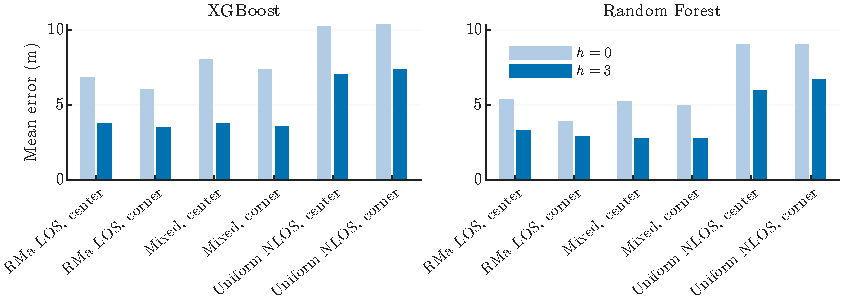
\includegraphics[width=0.95\textwidth]{fig_grid_mae}
  \caption{Controlled grid: mean position error from RSS and SINR at $h=0$ and $h=3$, per classifier, propagation setting and BS placement. Single run per bar.}
  \label{fig:grid-mae}
\end{figure}
% src: figure_scripts/fig_grid_mae.m (MATLAB); data/grid_comparison_sets.csv (= controlled_grid_2026_10/comparison_sets.csv)

% src: comparison_sets.csv (aoa_gain_pp BASE_H3 -> BASE_A_H3, XGBoost: centre 20.9 / 19.5 / 38.5; NE 4.0 / 1.0 / 6.2; history gain with AoA in m: centre 0.21-0.61, NE 0.74-2.03); results_summary.csv of centre_bs_mixed_30 (device parameters: XGB 59.2 -> 66.7 %, RF 65.7 -> 71.8 %)
The BS placement decides how much the angle is worth, whereas history helps at both placements. With history already in the input, adding AoA raised XGBoost's accuracy by $19.5$ to $38.5$ points with the BS at the center but by only $1.0$ to $6.2$ points beyond the corner, from where the whole grid falls within a wedge of about \ang{52} that a \ang{5} codebook barely resolves. Correspondingly, with AoA available, history lowers the error more beyond the corner~($0.7$ to \SI{2.0}{\meter}) than at the center~($0.2$ to \SI{0.6}{\meter}), where the angle already leaves little error to remove. Because RSS and SINR are stacked in absolute form, history could also be helping only by identifying the device; however, supplying the device parameters directly leaves a history gain of $6$ to $8$ points on top of them.

\subsection{The $25\times25$ Regression Runs}
\label{subsec:gain-regression}

% src: docs/results_of_record/regression_25x25_2026_10/{umilos,nlos,mixed}_30_fixednoise/{tuned,segment_shuffle}/results_summary.csv and sequence_vs_trees/all_mae.md (UMi LOS RF 14.52 -> 17.06, shuffled 14.73 -> 18.32; XGB 29.39 -> 13.72; NLOS XGB 33.25 -> 24.51, RF 29.32 -> 26.61; mixed XGB 29.89 -> 20.46, RF 24.33 -> 23.19); features_test (RF hybrid 8.14 vs 8.85; mixed 11.96 vs 11.75)
The $25\times25$ regression runs, which pool five simulated device profiles and test on the later part of each walk, show the same result at the macro-cell geometry~(Figure~\ref{fig:single-user}): without an angle, the best model with history beats the best snapshot model under all three propagation settings, and with the GRU of Section~\ref{sec:results-window} it does so with an angle as well~(Table~\ref{tab:cross-study}). The gain is not universal across models. On UMi LOS data Random Forest's error rose with three steps of history, under a chronological split and when the walk was cut into shuffled five-step blocks to prevent memorization of the path, while XGBoost's fell sharply from a snapshot model about twice as poor.\footnote{Replacing the stacked absolute lags with differences from the current snapshot removed Random Forest's loss in a related configuration with AoA, which points to its feature subsampling as the cause, but did not help on the mixed set.} Under uniform NLOS and mixed propagation both ensembles gain.

\begin{figure}[t]
  \centering
  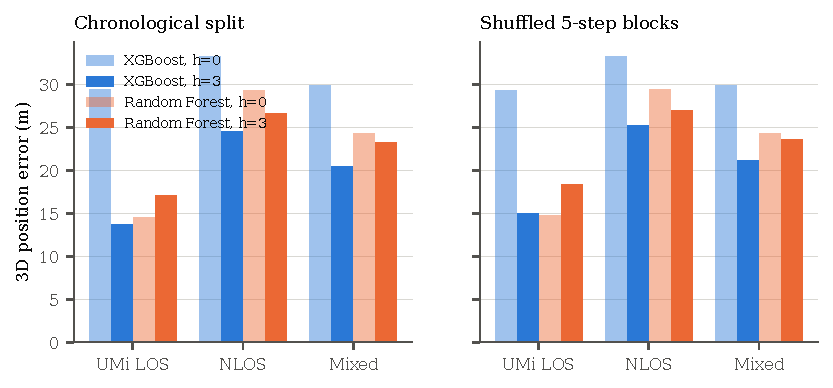
\includegraphics[width=0.85\textwidth]{fig_regression25_no_aoa}
  \caption{$25\times25$ regression with RSS and SINR only: mean position error at $h=0$ and $h=3$ for XGBoost and Random Forest, under a chronological and a block-shuffled split. Single run per bar; the shuffled split cuts each walk into five-step blocks.}
  \label{fig:single-user}
\end{figure}
% src: figure_scripts/python/make_figures_followup.py regression25_no_aoa(); docs/results_of_record/regression_25x25_2026_10

\subsection{The Macro Cell}
\label{subsec:gain-macro}

% src: data/seed_repeats_uniform_nlos.json (five splits; k-NN, GRU, 1D-CNN, mask-aware 1D-CNN, 1D-CNN + attention) and data/followup20_uniform_nlos.json (20 splits; XGBoost, RF); recomputed by figure_scripts/fig_history_gain_ci.m: multi-antenna gains 2.75 (RF) to 4.06 m (attention), 14.6-20.8 %; all Student-t intervals clear of zero
For multi-antenna devices in the macro cell, history lowered the error of every one of the seven model families, by $2.8$ to \SI{4.1}{\meter}, or $15$ to \SI{21}{\percent} of each model's own $h=0$ error~(Figure~\ref{fig:history-gain-ci}; per-model values in Table~\ref{tab:history-gain}). Every interval is clear of zero. The gain is of similar size across instance-based, bagged, boosted, recurrent, convolutional and attention-based models, so it comes from information that the $h=0$ input lacks and does not depend on the inductive bias of one architecture. These gains are measured under the angle impairment of Section~\ref{subsec:device-model}, in which every report carries an independent \ang{4} error; Section~\ref{subsec:averaging} examines how much of the gain depends on this independence.

\begin{figure}[t]
  \centering
  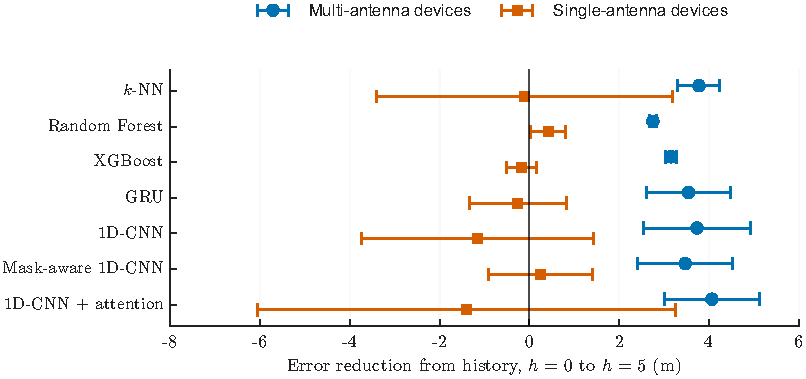
\includegraphics[width=0.8\textwidth]{fig_history_gain_ci}
  \caption{Macro cell, uniform NLOS: reduction in mean error from $h=0$ to $h=5$ per model and device group. Seed-paired means with \SI{95}{\percent} Student-$t$ intervals over $20$ user splits~(XGBoost, Random Forest) or five~(other models).}
  \label{fig:history-gain-ci}
\end{figure}
% src: figure_scripts/fig_history_gain_ci.m (MATLAB); data/seed_repeats_uniform_nlos.json, data/followup20_uniform_nlos.json

% src: data/macro_uniform_nlos_errors_seed42.csv (from diagnostics_2026_10/baseline_uniform_nlos/errors_first_seed.npz, seed 42) via figure_scripts/fig_macro_error_map.m: XGBoost multi 18.99 -> 15.41 m, single 34.66 -> 34.71 m; per-grid-point means: history lowers the multi-antenna error at 83 % of points (single 44 %); single-antenna h=5 error 22.6 m within 20 m of the area centre, 50.5 m beyond 40 m
Figure~\ref{fig:macro-error-map} shows where the errors fall. For multi-antenna devices the error is spread fairly evenly over the area, and history lowers it at \SI{83}{\percent} of the grid points. For single-antenna devices the error is lowest around the middle of the area and largest along its edges, with or without history, which is the pattern expected of predictions drawn toward the mean position.

\begin{figure}[t]
  \centering
  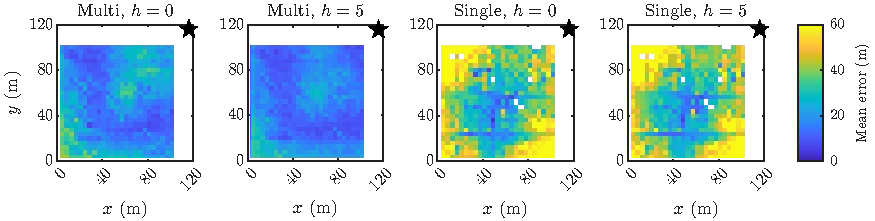
\includegraphics[width=\textwidth]{fig_macro_error_map}
  \caption{Macro cell, uniform NLOS: mean position error per grid point, XGBoost at $h=0$ and $h=5$, per device group, one user split. The star marks the serving BS.}
  \label{fig:macro-error-map}
\end{figure}
% src: figure_scripts/fig_macro_error_map.m (MATLAB); data/macro_uniform_nlos_errors_seed42.csv

% src: seed_repeats_all_models_summary.json ranking (h=5 overall, ranks 1-6 18.810-19.275); master_benchmark_rerun_summary.json (XGBoost 4 s training); xgb_per_h_retune_summary.json, rf_per_h_retune_summary.json (XGBoost tuning <= 0.44 m; RF < 0.07 m); followup_2026_10/history_depth (XGB full +1.21, +2.53, +3.15, +3.51, +3.68 at h = 1, 3, 5, 10, 20; 10-20 seeds); rts_retune_all_models_summary.json (RTS 2.5-4.7 %, test-tuned, backward pass)
With history in place, the choice of model matters far less than the input. At $h=5$ the six trained models other than $k$-NN fall within \SI{0.47}{\meter} of each other in overall error, and XGBoost reaches that level in \SI{4}{\second} of training. Re-tuning XGBoost and Random Forest separately at every depth, on training users only, changed their errors by at most \SI{0.44}{\meter} and left the history gain essentially unchanged~(Table~\ref{tab:supp-retune}), so the gain does not depend on hyperparameters chosen for one input size. The gain builds over the first steps of history~(Figure~\ref{fig:history-by-group} in Appendix~\ref{app:supplementary}): for XGBoost one extra report is worth \SI{1.2}{\meter}, and most of the gain is in place by ten.

\subsection{Propagation, Blockage and Interference}
\label{subsec:robustness}

% src: data/seed_repeats_mixed.json and data/followup20_mixed.json via figure_scripts/fig_history_gain_ci.m (multi-antenna gains 2.36 (RF) to 3.89 m, all intervals clear of zero; single-antenna XGB +1.14 +- 0.29, RF +1.28 +- 0.37, others span zero); seed_repeats ranking h=5 16.98-17.34 for ranks 1-6
\noindent\textbf{Mixed LOS and NLOS propagation.} Giving the four regions of the macro cell their own LOS or NLOS propagation leaves the multi-antenna result intact~(Figure~\ref{fig:mixed-gain}). History lowered the error of all seven families, by $2.4$ to \SI{3.9}{\meter}, and the six trained models other than $k$-NN again lie within \SI{0.4}{\meter} of each other. The single-antenna result differs from that of uniform NLOS, since both tree ensembles now gain $1.1$ to \SI{1.3}{\meter}; Section~\ref{subsec:mixed-single} examines where that gain arises. History also helps more in the regions that carry LOS propagation, but the same regions show the same difference in the uniform-NLOS realization, which contains no LOS at all; the difference is therefore a property of the regions, which lie in the range bands with the most error to remove, and not of LOS propagation~(Appendix~\ref{app:propagation}).
% src: followup_2026_10/mixed_propagation/region_gain_did_vs_uniform.json (20 seeds: gap 1.81 +- 0.27 uniform vs 1.54 +- 0.24 mixed; difference -0.27 +- 0.25; RF -0.01 +- 0.18)

\begin{figure}[t]
  \centering
  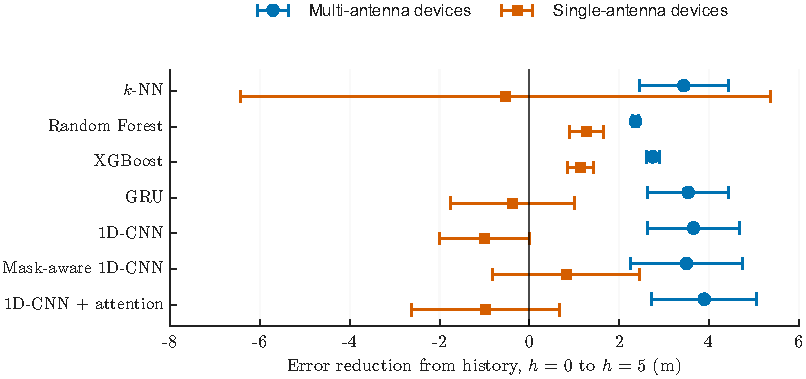
\includegraphics[width=0.8\textwidth]{fig_mixed_history_gain_ci}
  \caption{Macro cell, mixed propagation: reduction in mean error from $h=0$ to $h=5$ per model and device group. Seed-paired means with \SI{95}{\percent} Student-$t$ intervals over $20$ user splits~(XGBoost, Random Forest) or five~(other models).}
  \label{fig:mixed-gain}
\end{figure}
% src: figure_scripts/fig_history_gain_ci.m (MATLAB); data/seed_repeats_mixed.json, data/followup20_mixed.json

% src: CONTINUE_HERE.md §4 (prediction); followup_2026_10/blocked_los/history_mechanism_followup_summary.json (20 seeds, 360 users; multi-antenna XGBoost: blocked +6.29 +- 0.18 m (36.1 %), unblocked +6.66 +- 0.15 (38.7 %); by width +5.24 .. +6.11 m for 5-120 m, +7.65 m at 150 m; angle_mean blocked +6.51 +- 0.18; single-antenna blocked +0.47 +- 0.54)
% src: configs/b6_los_blocked_los_config.jsonc (corridor length 200 m; strip widths 5-150 m; speeds 1.5, 4.0, 10.0 m/s; BS [100,500,10]; UMi LOS / UMi NLOS); CONTINUE_HERE.md §4 (360 users, constant-range rationale)
\noindent\textbf{A blocked line of sight.} The fourth deployment follows UEs walking a straight \SI{200}{\meter} corridor whose middle section passes behind an obstruction, so that the link goes from LOS to NLOS and back; the width of the blocked strip varies from $5$ to \SI{150}{\meter}, and the BS stands \SI{500}{\meter} from the corridor so that the range is nearly constant along it. The scenario was designed to test whether history becomes more valuable as a blockage lengthens, up to the point where the heading observed before the blockage stops being informative. Over $20$ splits, history lowered the error of multi-antenna devices by \SI{36}{\percent} inside the blocked stretch and by \SI{39}{\percent} outside it for XGBoost, and the reduction does not rise and fall with the width of the blocked strip~(Figure~\ref{fig:blocked}), so the predicted dependence on blockage length does not appear. At that distance an azimuth step of \ang{5} spans tens of meters, and the unordered mean of the angle window recovers all of the gain, as in the macro cell. History thus keeps its value through a blockage of every length tested. Single-antenna devices gain nothing detectable in this scenario, inside or outside the blocked stretch.

\begin{figure}[h]
  \centering
  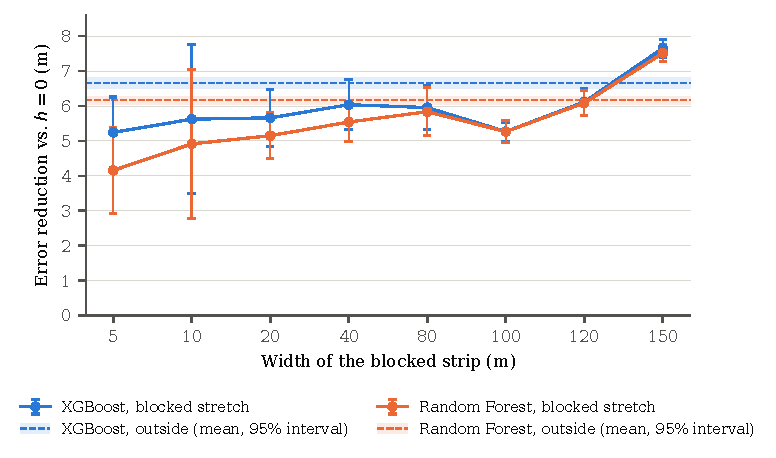
\includegraphics[width=0.7\textwidth]{fig_blocked_by_width}
  \caption{Blocked line of sight: reduction in multi-antenna error from $h=0$ to $h=5$ inside the blocked stretch, by strip width, with the mean outside it as a band. Seed-paired means over $20$ user splits with \SI{95}{\percent} Student-$t$ intervals.}
  \label{fig:blocked}
\end{figure}
% src: figure_scripts/python/make_figures_followup.py blocked_by_width()

% src: followup_2026_10/no_interference/{uniform_nlos,mixed_propagation}/history_mechanism_followup_summary.json (20 seeds; median SINR -3.0 dB; multi-antenna gain larger without interferers by 0.29-0.44 m; single mixed XGB 1.04 +- 0.23 vs 1.14 +- 0.29)
\noindent\textbf{Without the interfering BSs.} Both macro-cell realizations are interference-limited, with a median SINR of \SI{-3}{\decibel}. Switching the interferers off amounts to replacing SINR by the signal-to-noise ratio computed from the stored RSS. Over $20$ splits the multi-antenna history gain is slightly larger without them, by $0.3$ to \SI{0.4}{\meter}, and the single-antenna gain under mixed propagation is unchanged~(Table~\ref{tab:no-interference}); the conclusions do not depend on the interferers.

\section{Results: How Models Use the Window}
\label{sec:results-window}

As shown in Section~\ref{sec:results-gain}, history helps every model family; the families differ, however, in how long a window they can use. In this section, we compare tree ensembles and sequence models over windows of up to fifteen reports on the controlled grid and in the $25\times25$ runs, test whether the order of the reports matters, and compare the learned models with a classical tracking filter.

% src: docs/results_of_record/history_extended/ne_mixed/history_extended_summary.csv (XGB BASE 3.577 (h=3) -> 3.465 (h=15); RF 2.785 (h=3) -> 3.350 (h=15); CNN 8.339 (h=0) -> 2.486; GRU 1.424 at h=15, three seeds; BASE_A GRU 1.300, XGB 2.817, RF 3.146); centre_mixed (GRU BASE_A h=15 0.599, XGB 0.99); ne_mixed_lstm (1.399 vs 1.424); technical_documentation_revised.md 6.2 (GRU below the best tree in all eight set x AoA rows); RMa LOS accuracy, GRU h=15 (history_extended centre/ne_rmalos) vs RF h=3 (comparison_sets.csv): centre 51.0 vs 55.3 % (MAE 2.19 vs 3.32 m), NE 47.9 vs 55.4 % (2.48 vs 2.92 m); with AoA centre 68.5 vs 69.0 % (1.01 vs 1.38 m), NE 51.5 vs 58.2 % (1.87 vs 2.20 m); CLAIM_EVIDENCE_MAP.md C3 caveat
\noindent\textbf{Long windows.} The tree ensembles take their gain at one to three steps and then stop, whereas a GRU keeps improving with every added step up to $h=15$, and a 1D-CNN does so in most settings~(Figure~\ref{fig:history-extended}). In the mixed setting with the BS beyond the corner and without AoA, XGBoost is flat from $h=3$ on and Random Forest is worse at fifteen steps than at three, while the GRU reaches \SI{1.42}{\meter} against $3.35$ and \SI{3.46}{\meter} for the two trees. The same ordering holds with AoA and in all four combinations of propagation setting and placement tested, so that the ranking of the families at long history is the reverse of their ranking at no history. The GRU's advantage lies in mean error: on the RMa LOS sets, Random Forest at three steps matches or exceeds the GRU's accuracy at fifteen, while its mean error remains higher. A long short-term memory~(LSTM) network of the same size performs the same as the GRU~($1.40$ against \SI{1.42}{\meter}), so the gain comes from the sequence, not from the recurrent cell.

\begin{figure}[h]
  \centering
  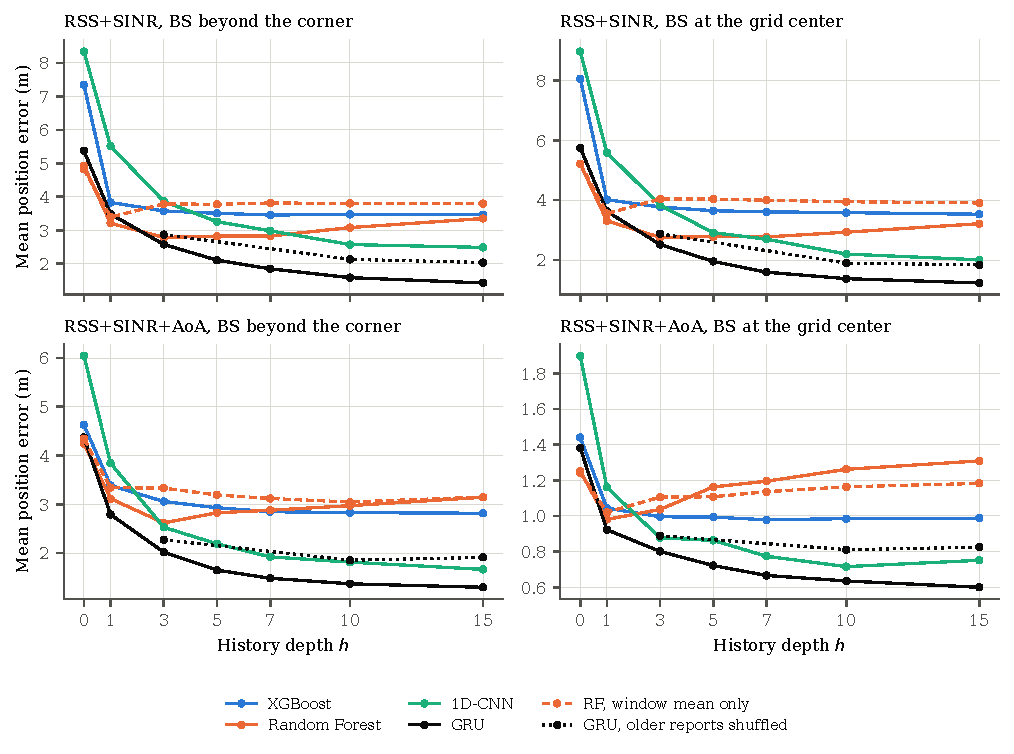
\includegraphics[width=0.95\textwidth]{fig_history_extended}
  \caption{Controlled grid, mixed propagation: mean position error against history depth $h$, without and with AoA, per BS placement. Trees and window-mean trees: single run; CNN and GRU: three seeds; shuffled GRU: two seeds.}
  \label{fig:history-extended}
\end{figure}
% src: figure_scripts/python/make_figures_followup.py history_extended_fig()

% src: docs/results_of_record/regression_25x25_2026_10/sequence_vs_trees/all_mae.md (GRU h=15 three seeds, spread <= 0.4 m; 1.3-5.0 m below the best tree at any depth; trees tuned at h=3; 400-epoch cap lowers the error by up to 0.9 m)
The $25\times25$ runs repeat the pattern at the macro-cell geometry. A two-layer GRU over the last $h+1$ reports keeps improving up to $h=15$ and has the lowest error in all six combinations of propagation setting and angle, $1.3$ to \SI{5.0}{\meter} below the best tree model at any depth~(Table~\ref{tab:cross-study}), while a 1D-CNN follows the same course slightly above it. History therefore lowers the error of the best model in this setting as well. The tree models use parameters tuned at $h=3$ and the GRU was still improving at its epoch limit, so the size of the gap is approximate.

% src: PLAN_AND_CHECKLIST.md 12.4 (window-mean trees; XGB h=5 4.52 vs 3.51 m); docs/results_of_record/history_extended/order_test_comparison.csv and technical_documentation_revised.md 6.2 table (older reports shuffled, current report kept, two seeds; GRU h=15 increase 19.0 % (RMa LOS NE, no AoA) to 49.0 % (mixed centre, no AoA, 1.235 -> 1.841 m); ne_mixed 1.424 -> 2.033 m; shuffled GRU below the best tree in 8/8 rows)
\noindent\textbf{The order of the reports.} Two controls show what the sequence models use. Giving the trees only the current report and the mean of the window does not make them keep improving; without AoA they are worse than the trees on raw lags from $h=3$ on. Permuting the older reports inside each window, in training and in test, while the current report keeps its place, raises the error of the GRU at $h=15$ by $19$ to \SI{49}{\percent} in all eight combinations of set, placement and angle, and the shuffled network gains little beyond ten steps while the ordered one keeps gaining. The shuffled GRU is nevertheless still more accurate than the best tree in all eight combinations, so only part of its advantage depends on order. We attribute this to the distance-ring ambiguity: a single RSS and SINR report is ambiguous between cells on the same signal contour around the BS, the mean of a window does not remove that ambiguity, and the ordered sequence of reports, which traces the movement across the contours, does. The history gain on the grid would then have two parts: an averaging part, shared by all models and the only part isolated in the macro cell~(Section~\ref{sec:results-mechanism}), and a sequence part that only recurrent and convolutional models exploit.

% src: results_of_record/tracking_filter/ne_mixed/tracking_filter.csv (RF snapshot 4.927 m; filter learned 0.714 m; generic 2 m kernel 0.93 m), technical_documentation_revised.md 6.2 l.261-278 (causal HMM forward filter; transition matrix learned from the training walks; caveats); history_irregular/ne_mixed{,_cnn}/history_irregular_summary.csv; paper/tables/T5_grid_baselines.md; CLAIM_EVIDENCE_MAP.md C8 (GRU keeps 80-90 % of its gain), C9
\noindent\textbf{A tracking filter and imperfect history.} History can also be used through a motion model instead of a learned window. A hidden Markov model~(HMM) forward filter on top of the Random Forest snapshot model combines the previous cell probabilities, propagated by a transition matrix, with those of the current report, and uses past reports only. With a transition matrix learned from the training walks, or with a generic kernel over distance, it lowers the error below that of the GRU~(Table~\ref{tab:grid-baselines}). The grid walk moves to a neighboring cell at every step and at constant speed, which a motion model suits well; the filter is therefore reported as a classical history-based baseline, and it was not run on the less regular trajectories of the macro cell. The learned models also tolerate imperfect history: when the older reports are missing at random or arrive at uneven gaps, and the models are trained with the same imperfection, the GRU keeps $80$ to \SI{90}{\percent} of its gain over the snapshot model and remains more accurate than XGBoost with complete history.

\begin{table}[h]
  \centering
  \caption{Controlled grid, mixed propagation, BS beyond the corner, RSS and SINR: mean position error~(m) with complete and imperfect history.}
  \label{tab:grid-baselines}
  \small
  \begin{tabular}{@{}llccc@{}}
    \toprule
    Model & Use of history & Complete & \SI{30}{\percent} missing & Uneven gaps \\
    \midrule
    Random Forest, current report only & none & $4.93$ & $4.90$ & $4.93$ \\
    XGBoost, $10$ older reports & learned window & $3.45$ & $4.07$ & $3.93$ \\
    1D-CNN, $10$ older reports & learned sequence & $2.49$ & $3.38$ & $3.01$ \\
    GRU, $10$ older reports & learned sequence & $1.59$ & $2.06$ & $1.99$ \\
    Random Forest + HMM, generic motion & motion model & $0.93$ & $1.16$ & $1.41$ \\
    Random Forest + HMM, learned motion & motion model & $0.71$ & $0.98$ & $1.27$ \\
    \bottomrule
  \end{tabular}
\end{table}
% src: paper/tables/T5_grid_baselines.md (uneven gaps: mean 2 steps; learned models trained with the same imperfection; CNN three seeds, GRU two, others single run)

\section{Results: What History Reads in the Macro Cell}
\label{sec:results-mechanism}

In this section, we identify which part of the macro-cell input carries the history gain of Section~\ref{subsec:gain-macro}, and what that part contains. All comparisons share the samples and user splits of the full $h=5$ input, so each comparison is paired.

% src: followup_2026_10/uniform_nlos/history_mechanism_followup_summary.json summary.{xgboost,random_forest}.{angle_hist,rss_hist,ray_hist,full}.multi.gain_vs_snap.all (20 seeds, Student-t: angle 3.16 +- 0.14 / 3.06 +- 0.13; full 3.15 +- 0.12 / 2.75 +- 0.08; rss 0.23 +- 0.09 / -0.22 +- 0.11; ray 0.25 +- 0.11 / -0.01 +- 0.10); diagnostics_2026_10/baseline_uniform_nlos (k-NN, five seeds: angle 5.19, full 3.79, rss -2.27); diagnostics_2026_10/mixed_propagation (angle-only 2.4-3.6 m, three models); followup_2026_10/neural_uniform_nlos (five seeds: angle_hist 3.11/3.43/3.27/2.98; full 3.07/3.19/3.19/2.85; rss_hist 0.17/0.19/0.16/0.16)
\noindent\textbf{The angle channels.} The test feeds a model history for one group of channels at a time while holding every other channel at its current value: the RSS group~(RSS, SINR and the RSS difference), the angle group~(the sines and cosines of both angles and the azimuth difference), or the ray group~(the two ray-projection coordinates and their differences). For multi-antenna devices on the uniform-NLOS data, angle history alone gives as much as history on every channel, over $20$ splits $3.16$ against \SI{3.15}{\meter} for XGBoost and $3.06$ against \SI{2.75}{\meter} for Random Forest, whereas RSS history and ray history give at most \SI{0.25}{\meter}~(Figure~\ref{fig:angle-decomposition}). The same holds for the other five families over five splits: for $k$-NN angle history alone outperforms the full window, because the RSS lags, which alone raise its error, add noise to its distance metric, and for the four neural models angle history alone lowers the error by $3.0$ to \SI{3.4}{\meter} and RSS history by under \SI{0.2}{\meter}. The mixed-propagation data repeat the pattern. The result therefore covers all seven model families.

% src: followup_2026_10/uniform_nlos summary.xgboost.{snap,full}.multi.shape (20 seeds: radial 17.21 -> 14.06, tangential 4.96 -> 4.61; RF 17.39 -> 14.77, 4.65 -> 4.15); summary.{xgboost,random_forest}.pure_snap.multi.gain_vs_snap.all (20 seeds: -0.56 +- 0.16 / -0.37 +- 0.08)
What the angle history improves is mainly the estimate of distance. For multi-antenna devices, five steps of history lowered XGBoost's mean radial error from $17.2$ to \SI{14.1}{\meter} but its tangential error only from $5.0$ to \SI{4.6}{\meter}, and Random Forest behaves alike; bearing is already well determined by the current angle, and the window improves range. It should be noted that the $h=0$ input already holds one step of change through its first differences: removing them raises the multi-antenna error by \SI{0.56}{\meter} for XGBoost and \SI{0.37}{\meter} for Random Forest, so the gains reported here understate the full effect of history by roughly \SI{15}{\percent}.

\subsection{What the Angle History Contains}
\label{subsec:averaging}

% src: followup_2026_10/uniform_nlos (20 seeds, XGBoost / RF, multi-antenna, Student-t): full 3.15+-0.12 / 2.75+-0.08; angle_hist 3.16+-0.14 / 3.06+-0.13; angle_mean 3.38+-0.19 / 3.61+-0.19; angle_shuffled 2.93+-0.12 / 2.66+-0.13; el_hist 2.72+-0.13 / 2.24+-0.12; az_hist 0.63+-0.08 / 0.77+-0.05
Section~\ref{subsec:history-dof} sets out two ways in which a window of angles can carry position: through its rate of change, since for a given sideways movement the bearing turns at the rate $v_\perp/r$, or through repeated noisy samples, since every angle report is the true angle plus an independent \ang{4} error quantized to \ang{5} steps, and averaging several reports of a nearly unchanged angle gives a better estimate. Four tests over $20$ splits separate the two~(Figure~\ref{fig:angle-decomposition}): (i)~replacing the window by the unordered mean of each angle channel gives as much as the ordered history; (ii)~shuffling the order of the earlier reports costs only $0.2$ to \SI{0.4}{\meter}; (iii)~elevation history alone gives most of the gain; and (iv)~azimuth history alone gives under \SI{0.8}{\meter}. The BS stands about \SI{8.5}{\meter} above a device, so elevation encodes distance, and averaging it improves the range estimate; this is why it is the radial error that falls with history.

\begin{figure}[h]
  \centering
  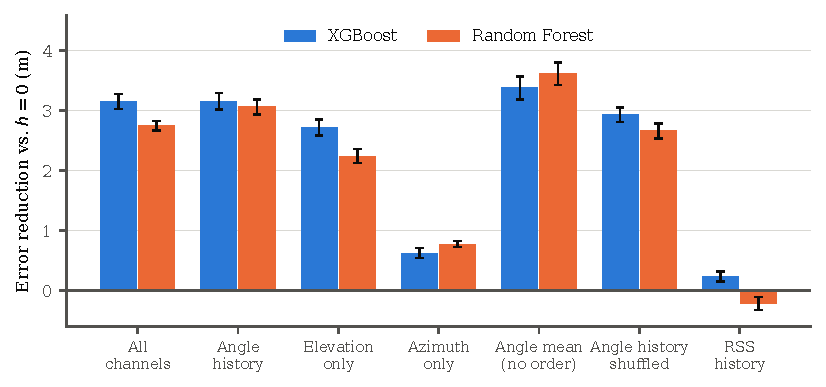
\includegraphics[width=0.95\textwidth]{fig_angle_decomposition}
  \caption{Macro cell, uniform NLOS: reduction in multi-antenna error from $h=0$ to $h=5$ when history is given for all channels, parts of the angle information, or RSS only. Seed-paired means over $20$ user splits with \SI{95}{\percent} Student-$t$ intervals.}
  \label{fig:angle-decomposition}
\end{figure}
% src: figure_scripts/python/make_figures_followup.py angle_decomposition()

% src: followup_2026_10/aoa_impairment/{clean,quant5_only,noise4_only,noise8_quant5} (10 seeds, full history, multi-antenna; clean: XGB h=0 2.32 m, RF 1.58 m, gain +0.00 +- 0.11 / -1.02 +- 0.03; quantization only: h=0 14.2 m, gain 1.9 / 2.3 m; noise only 3.1 m); neural_exact_aoa (gain -0.48 to -0.78 m; h=0 error 1.8-3.2 m)
The decisive test removes the error. With exact arrival angles the multi-antenna error without history falls to between $1.6$ and \SI{3.2}{\meter} across the six models tested, and history adds nothing for XGBoost and makes Random Forest and the four neural models worse: there is nothing left to average. Quantization alone, or noise alone, still leaves a gain~(Figure~\ref{fig:aoa-error-model}a). The history gain of Section~\ref{subsec:gain-macro} is thus a property of averaging imperfect angle reports, not of bearing geometry.

\begin{figure}[h]
  \centering
  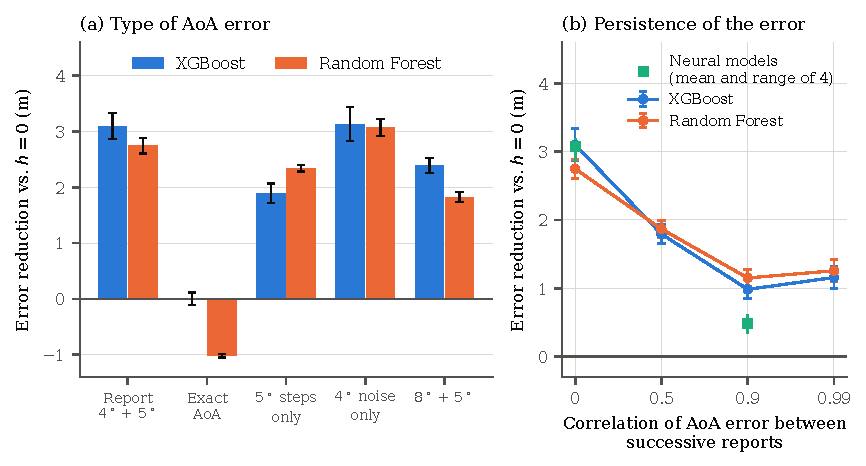
\includegraphics[width=0.95\textwidth]{fig_aoa_error_model}
  \caption{Macro cell, uniform NLOS: reduction in multi-antenna error from $h=0$ to $h=5$ under (a)~different types of angle error and (b)~a \ang{4} error correlated between successive reports. Ten user splits per point, five for the neural models; \SI{95}{\percent} Student-$t$ intervals.}
  \label{fig:aoa-error-model}
\end{figure}
% src: figure_scripts/python/make_figures_followup.py aoa_error_model()

% src: followup_2026_10/aoa_impairment/corr_rho{0,0.5,0.9,0.99} (10 seeds; XGB full +3.10, +1.79, +0.98, +1.16; elevation +2.69 -> +0.03; RF +2.75 -> +1.26); neural_corr_rho0.9 (+0.34 to +0.61 m, 2-3 %)
How much of the gain remains depends on how the error behaves from one report to the next. If the angle error persists across the window, averaging cannot remove it. Making the \ang{4} error an autoregressive sequence along each walk, XGBoost's gain falls from \SI{3.1}{\meter} with independent errors to about \SI{1}{\meter} at lag-1 correlations of $0.9$ and above~(Figure~\ref{fig:aoa-error-model}b). The elevation part disappears first; what remains, $5$ to \SI{7}{\percent} of the error, is in azimuth, and the neural models keep only $2$ to \SI{3}{\percent}. The headline gain of $15$ to \SI{21}{\percent} is therefore specific to angle errors that are independent between reports, which is how the macro-cell simulation draws them.

% src: followup_2026_10/history_depth/h{1,3,10,20} (10 seeds) and uniform_nlos (h=5, 20 seeds), XGBoost multi-antenna full +1.21, +2.53, +3.15, +3.51, +3.68; angle_mean +1.26, +2.72, +3.38, +3.16, +1.39; angle_hist at h=20 +3.59
The same account explains how the gain depends on window length. The unordered mean of the angle window is the better input up to five steps and then fails, falling to \SI{1.4}{\meter} at twenty steps, because over \SI{80}{\meter} of travel the true angle has changed and an unweighted mean is biased; the ordered window still gives \SI{3.6}{\meter} there, since the model can weight recent reports. At long windows the order of the reports does matter in the macro cell, for discounting stale ones.

\section{Results: When History Adds Nothing}
\label{sec:results-no-gain}

In this section, we examine the one setting of Table~\ref{tab:cross-study} in which history does not help, single-antenna devices in the macro cell, and test two explanations for it: the range of the macro cell and the fact that its test users were not seen in training.

% src: followup_2026_10/uniform_nlos/history_mechanism_followup_summary.json summary.{xgboost,random_forest}.full.single.gain_vs_snap.all (20 seeds, Student-t: XGB -0.18 +- 0.34, RF +0.42 +- 0.39, 1.1 %); fig_history_gain_ci.m output (five-split families: all single-antenna intervals span zero); single_share_50/uniform_nlos (20 seeds: XGB +0.30 +- 0.24, RF +0.18 +- 0.24); followup20 user_counts (3-11 single-antenna test users per split, mean 6.85)
For single-antenna devices in the macro cell, history produced no meaningful change in error in any of the seven model families~(Figure~\ref{fig:history-gain-ci}). Over $20$ splits XGBoost's error rises by \SI{0.18 +- 0.34}{\meter} and Random Forest's falls by \SI{0.42 +- 0.39}{\meter}, about \SI{1}{\percent}, and the intervals of the five other families, over five splits, all span zero; the same seven models gained $15$ to \SI{21}{\percent} on multi-antenna devices drawn from the same test users. Each split holds only $3$ to $11$ single-antenna test users, which is why their intervals are wider; with half of the devices single-antenna, the gain is at most \SI{0.3}{\meter}. History therefore gives these devices no more than about \SI{1}{\percent} on uniform-NLOS data.

% src: naive_baseline/uniform_nlos (20 seeds: single 38.50); followup_2026_10/uniform_nlos summary.xgboost.snap.single (36.33 m; shape: radial_share_sq 0.41, range_corr 0.51 +- 0.06, radial_bias -9.73); diagnostics_2026_10/baseline_uniform_nlos/errors_first_seed.npz (seed 42, XGBoost: user 250 bearing span 73 deg true, 17 deg predicted; user 27 65 vs 68 deg)
The reason is that a single report already carries almost nothing that the model can use for these devices. Always predicting the mean training position gives \SI{38.5}{\meter}, so a snapshot model at \SI{36.3}{\meter} has recovered only about \SI{6}{\percent} of the error, and history leaves that unchanged. The failure has the shape of the distance-ring ambiguity of Section~\ref{subsec:ambiguity-hypothesis}, but without the distance: about \SI{60}{\percent} of the squared error is tangential, the predicted range correlates only $0.51$ with the true range, and predictions are pulled toward the BS by about \SI{10}{\meter} on average. For the median single-antenna test user~(Figure~\ref{fig:trajectories} in Appendix~\ref{app:macro-errors}), the walk spans \ang{73} of bearing while the predicted positions, with or without history, span \ang{17}; those of the median multi-antenna user follow the shape of the walk closely.


\subsection{A Range-Dependent Explanation}
\label{subsec:hypothesis}

% src (derived): pathloss_fit_summary.json range_resolution fitted_db_per_m (1.4176 dB/m at 10 m; 0.1487 dB/m at 95 m) x step length (2 m controlled grid; 4 m macro cell); sigma 10.1 dB; angular: 4 m / 95 m rad = 2.4 deg vs 4 deg Gaussian + 5 deg codebook (csi_dataset.py)
% src: followup_2026_10/uniform_nlos (20 seeds): single rss_hist XGB +0.02 +- 0.37, RF +0.29 +- 0.44; multi rss_hist by range XGB 0.93, 0.63, -0.15, 0.70 m, RF no trend (-1.39, 0.43, -0.42, -0.37); followup_2026_10/mixed_propagation single rss_hist XGB by range 1.76, 0.90, 1.34, 1.48 m
The contrast with the controlled grid and the $25\times25$ runs, where RSS and SINR history did help, has a candidate explanation in Equation~(\ref{eq:rss-gradient}): the RSS change produced by one step shrinks with distance from the BS, from about \SI{2.8}{\decibel} for a \SI{2}{\meter} step at \SI{10}{\meter} to about \SI{0.6}{\decibel} for a \SI{4}{\meter} step at the macro cell's median range of \SI{95}{\meter}, against shadowing with a spread of \SI{10}{\decibel}, whereas the bearing still turns by about \ang{2.4} per sideways step there. The account predicts that (i)~angle history carries the multi-antenna gain; (ii)~no part of the history lowers the single-antenna error; and (iii)~any gain from RSS history falls with range. The first prediction holds~(Section~\ref{sec:results-mechanism}); the second holds under uniform NLOS but fails under mixed propagation~(Section~\ref{subsec:mixed-single}); and the third is not supported, since XGBoost's RSS-only gain falls and then rises again with range and Random Forest's has no trend. The range account therefore does not explain when RSS history helps; only its angle half is confirmed.

% src: CLAIM_EVIDENCE_MAP.md C5 "Result of test (a)" and "Consequences" (2026-10-24); results_of_record/leave_one_user_out/ne_mixed/leave_one_user_out_summary.csv (unseen user MAE 12.02-12.45 m, accuracy 0.7-1.1 %; GRU h=10 1.62 m on the time split, 12.38 m unseen); map_similarity.json (per-cell RSS correlation between users 0.02-0.83; U1-U4 0.02); constant guess 10.9 m
\subsection{Unseen Users}
\label{subsec:unseen-users}

The controlled grid and the $25\times25$ runs also differ from the macro cell in testing later parts of the walks of users seen in training. This difference was examined directly on the controlled grid~(mixed setting, BS beyond the corner, RSS and SINR), by training on four of the five device profiles and testing on the fifth. On an unseen user every model fails, with or without history: the mean error rises to about \SI{12}{\meter}, worse than the \SI{10.9}{\meter} of a constant guess, whereas the same GRU reaches \SI{1.6}{\meter} on the usual split. The users do not share a channel map; each is simulated as a separate channel realization, and the per-cell mean RSS of two users can be almost uncorrelated, even for identical device profiles. The controlled-grid results without an angle are therefore within-user results, in which a model learns each user's own map from the first part of the walk and history sharpens the use of that map. The $25\times25$ runs share this design, although the test was not repeated there. The macro-cell test users offer no such learned map, so single-antenna devices there have nothing for history to amplify. In a real deployment, co-located users share the large-scale shadowing, so the separate channel realizations of the simulation make this contrast sharper than it would be in practice; Section~\ref{subsec:shared-env} tests this with an environment shared by all users.

\subsection{The Exception: Single-Antenna Devices under Mixed Propagation}
\label{subsec:mixed-single}

% src: followup_2026_10/mixed_propagation summary.{xgboost,random_forest}.rss_hist.single.gain_vs_snap.{geo_LOS,geo_NLOS} (20 seeds: XGB 1.17 +- 0.32 / 1.46 +- 0.54; RF 1.18 +- 0.37 / 2.01 +- 0.50); followup_2026_10/mixed_propagation_los_flag (20 seeds, single-antenna: rss_hist XGB +1.28 +- 0.29, RF +1.41 +- 0.36; snap_los +3.27 / +3.04; history on top of flag +1.01 / +0.77; crossing windows +2.61 / +3.92, 14 % of windows; entirely LOS +0.79 / +0.34, entirely NLOS +0.63 / -0.03); single_share_50/mixed_propagation (+1.20 +- 0.15 / +1.42 +- 0.15); CONTINUE_HERE.md 1a (LOS-NLOS RSS gap 16.87 dB)
Under mixed propagation, history lowers the single-antenna error of both tree ensembles by $1.1$ to \SI{1.3}{\meter}, while the neural models and $k$-NN show no gain beyond their intervals~(Figure~\ref{fig:mixed-gain}). RSS history alone gives as much, $1.3$ to \SI{1.4}{\meter} over $20$ splits, positive in every split. The gain is not explained by the cleaner path-loss relation of LOS propagation, since it is at least as large in the NLOS regions as in the LOS ones. What it does depend on is the propagation state itself. A single-antenna snapshot cannot tell LOS from NLOS, which differ by about \SI{17}{\decibel} in RSS, and adding the true LOS flag to the snapshot as an oracle lowers the error by about \SI{3}{\meter}; RSS history recovers part of this, and given on top of the oracle flag it still gains $0.8$ to \SI{1.0}{\meter}, concentrated in the \SI{14}{\percent} of windows that span a crossing between regions. We attribute the gain to two effects of the window: it helps to infer the propagation state, and, at a crossing, it marks a place on the map where the signal strength steps.

% src: results_of_record/device_generalization_2026_11/{macro_mixed,macro_mixed_gru,shared,shared_gru,seed2_shared,seed2_shared_gru,macro_uniform,macro_uniform_gru,shared_uniform,shared_uniform_gru} device_generalization.csv (offset 0, groups multi/single, gain = snap - rep per seed, seeds 42-46, Student-t); *_class_gru_h20 summaries (cls_iot snap/diff); MANIFEST.md section device_generalization_2026_11; same-point |dP| median 5.1 vs 6.7 dB
\subsection{A Shared Environment}
\label{subsec:shared-env}

To test how much of the macro-cell result is due to simulating every user as a separate channel realization, we generated three further macro-cell datasets in which all users share one environment: two with the mixed LOS and NLOS regions of the macro cell, drawn from different seeds, and one in which every region is NLOS. Each has $300$ users in four device classes: mid-tier phones with four antenna elements, flagship phones and vehicles with sixteen, and single-antenna IoT devices, which differ in carrying height, antenna gain, noise figure and speed. The random generator of the channel simulation is reset to a common seed before every segment of every walk, so that all users see the same large-scale parameter maps; the small-scale fading is still drawn per segment, so the environment is only partly shared. At the same grid point, the median difference in received power between two users is \SI{5.1}{\decibel}, against \SI{6.7}{\decibel} with separate realizations. No angle is used in this comparison, and no static device attributes are given to the models.

Table~\ref{tab:shared-env} compares the history gain on unseen users~(five user splits, \SI{80}{\percent} of users for training) with separate realizations and in the shared environments, for XGBoost and a one-layer GRU given the last $h=5$ reports. With separate realizations, history lowers the error by $2$ to \SI{3}{\meter} under mixed propagation, in line with the single-antenna gain of Section~\ref{subsec:mixed-single}, and not at all under uniform NLOS; in both cases the differences between consecutive reports make the error worse than a single report. In the shared environments, the gain grows for both models and both propagation settings. It is largest for the GRU given levels and differences together, which lowers the error of multi-antenna devices by $9$ to \SI{10}{\meter}, and the differences between reports now lower the error as well. Under uniform NLOS, where history gains nothing with separate realizations, the shared environment gives single-antenna devices a gain of \SI{5.9 +- 3.2}{\meter} with the GRU; the gain of XGBoost, \SI{2.5 +- 2.0}{\meter}, is not clearly different from zero. With $h=20$ and the GRU trained on phones only, the differences alone bring single-antenna IoT devices, a class not seen in training, from $37.5$ and \SI{35.1}{\meter} to $20.2$ and \SI{21.1}{\meter} in the two mixed environments, and from $32.9$ to \SI{23.8}{\meter} under uniform NLOS.

A shared map therefore lets history, and above all the change between reports, carry over to new users. The uniform-NLOS result of this section, where history adds nothing for single-antenna devices, is thus largely a consequence of the separate realizations, although the single-antenna evidence rests on one model and one environment.

\begin{table}[h]
  \centering
  \caption{History gain on unseen users with separate channel realizations and in a shared environment~(macro-cell geometry, no angle). Error of a single report~($h=0$) and its reduction by a window of $h=5$ reports, in metres; seed-paired means over five user splits with \SI{95}{\percent} Student-t intervals. Levels: the reports as received; differences: the change between consecutive reports; both: the two together. Shared~1 and~2 are two environments drawn from different seeds.}
  \label{tab:shared-env}
  \small
  \begin{tabular}{@{}llllrrrr@{}}
    \toprule
    Propagation & Environment & Model & Devices & $h=0$ & Levels & Differences & Both \\
    \midrule
    Mixed & Separate & XGBoost & Multi  & $29.4$ & $2.3 \pm 0.6$ & $-3.3 \pm 0.4$ & $2.4 \pm 0.6$ \\
          &          &         & Single & $28.7$ & $2.6 \pm 0.5$ & $-2.9 \pm 1.3$ & $2.9 \pm 0.6$ \\
          &          & GRU     & Multi  & $28.3$ & $1.8 \pm 0.3$ & $-3.6 \pm 0.6$ & $2.1 \pm 0.8$ \\
          &          &         & Single & $27.8$ & $2.3 \pm 0.7$ & $-2.7 \pm 1.3$ & $2.9 \pm 0.6$ \\
    \cmidrule{2-8}
          & Shared 1 & XGBoost & Multi  & $30.6$ & $3.9 \pm 0.4$ & $-0.3 \pm 0.5$ & $4.6 \pm 0.4$ \\
          &          &         & Single & $32.1$ & $2.8 \pm 1.1$ & $-0.2 \pm 1.4$ & $3.5 \pm 0.8$ \\
          &          & GRU     & Multi  & $29.8$ & $5.2 \pm 0.7$ & $6.8 \pm 1.9$  & $9.0 \pm 1.3$ \\
          &          &         & Single & $32.1$ & $3.6 \pm 1.1$ & $5.4 \pm 3.7$  & $7.2 \pm 2.0$ \\
    \cmidrule{2-8}
          & Shared 2 & XGBoost & Multi  & $31.4$ & $4.1 \pm 0.5$ & $0.3 \pm 0.6$  & $5.8 \pm 0.6$ \\
          &          &         & Single & $31.0$ & $3.2 \pm 1.0$ & $-0.6 \pm 2.0$ & $4.1 \pm 1.3$ \\
          &          & GRU     & Multi  & $30.4$ & $6.2 \pm 1.1$ & $6.5 \pm 2.5$  & $8.9 \pm 1.8$ \\
          &          &         & Single & $30.7$ & $3.9 \pm 3.9$ & $4.1 \pm 4.9$  & $5.7 \pm 4.3$ \\
    \midrule
    NLOS  & Separate & XGBoost & Multi  & $33.7$ & $0.2 \pm 0.3$  & $-2.0 \pm 0.4$ & $0.4 \pm 0.3$ \\
          &          &         & Single & $33.4$ & $-0.2 \pm 0.6$ & $-2.3 \pm 1.2$ & $-0.2 \pm 0.7$ \\
          &          & GRU     & Multi  & $33.6$ & $0.3 \pm 0.3$  & $-2.1 \pm 0.4$ & $0.2 \pm 0.4$ \\
          &          &         & Single & $33.5$ & $-0.2 \pm 0.7$ & $-1.9 \pm 1.3$ & $0.0 \pm 0.5$ \\
    \cmidrule{2-8}
          & Shared   & XGBoost & Multi  & $34.2$ & $5.1 \pm 0.5$ & $1.1 \pm 0.6$  & $5.8 \pm 0.5$ \\
          &          &         & Single & $32.8$ & $2.0 \pm 2.0$ & $-0.7 \pm 2.6$ & $2.5 \pm 2.0$ \\
          &          & GRU     & Multi  & $32.6$ & $7.4 \pm 1.2$ & $5.1 \pm 2.0$  & $10.1 \pm 2.2$ \\
          &          &         & Single & $33.1$ & $3.8 \pm 3.1$ & $1.8 \pm 4.3$  & $5.9 \pm 3.2$ \\
    \bottomrule
  \end{tabular}
\end{table}

\section{Discussion}
\label{sec:discussion}

% src: Sections 5-8 (numbers as cited there); REPORT_SKELETON_VALIDATION.md (A1-A15); CLAIM_EVIDENCE_MAP.md C5 (common reading, test (a), consequences), C9
As shown in Sections~\ref{sec:results-gain}--\ref{sec:results-no-gain}, history lowers the error in every study, setting and model family but one. In this section, we discuss what history adds, when it helps and what this implies in practice, and then state the limitations of this work.

\noindent\textbf{What history adds.}
Section~\ref{subsec:history-dof} set out two ways in which a window can add to a single report: through the rates of change of the measurements, which require the reports in order, and through repeated noisy samples, which do not. In the macro cell, the gain comes from the second: the window averages out the error of the angle reports. On the controlled grid, the order of the reports also matters, so there the sequence models draw on the first mechanism as well.

\noindent\textbf{When history helps.}
The results fit one rule: history improves on whatever position information a single report already carries, and it cannot create information that is not there. With an angle, a single report locates the device in every study, and a window locates it better. Without an angle, a single report locates the device only where the model knows how the signal varies over the area for that device, as a fingerprinting system does once the area has been surveyed. The controlled grid and the $25\times25$ runs are of this kind: each model is trained on the first part of every walk and tested on the remainder, so it has in effect surveyed each device's radio map, and history sharpens its use of that map. Because the history gain is measured against the same model on the same split without history, the survey benefits both inputs equally. Without the survey, the same grid models fail~(Section~\ref{subsec:unseen-users}). The macro cell tests on users absent from training, so there a single-antenna report carries almost no usable information, and history adds nothing. The larger range of the macro cell does not explain this difference, since the RSS-history gain does not fall with range~(Section~\ref{subsec:hypothesis}). The one exception, single-antenna devices under mixed propagation, follows the same rule: there a window reveals whether the link is LOS or NLOS, something that no single report can show on its own.

\noindent\textbf{Practical case.}
For a deployment, the input matters more than the estimator. Once history is included, the trained models of the macro cell reach nearly the same error, and XGBoost, which trains in seconds, is among them. On the grid, a motion-model filter uses history better still, so the gain lies in the history itself and not in a particular learned model. Finally, the conditions that a deployment is most likely to vary, namely LOS propagation, a blocked line of sight and the interfering BSs, leave the gain intact.

\subsection{Limitations}
\label{subsec:limitations}

% src: FINAL_REPORT.md §9 items 1-5; Section III (QuaDRiGa, TR 38.901; four mobility patterns, 0.1-15 m/s)
\noindent\textbf{Simulation.} All results come from simulation. The channels are generated by a 3GPP TR~38.901-compliant simulator and the macro-cell users follow four mobility patterns at speeds from pedestrian to vehicular, but real channels add hardware impairments and calibration drift, and real movement follows roads and stops. Because every simulated step advances exactly one grid cell, history depth also measures the distance travelled, and the two effects are not separated here.

% src: followup_2026_10/aoa_impairment corr_rho0.9, corr_rho0.99 (10 seeds; trees 5.2-6.7 %, all intervals clear of zero); neural_corr_rho0.9 (+0.34 to +0.61 m, 2-3 %); followup_2026_10/uniform_nlos single (20 seeds, intervals +-0.34 / +-0.39 m; 3-11 single-antenna test users)
\noindent\textbf{Angle error and device mix.} The \SIrange{15}{21}{\percent} macro-cell gain assumes angle errors that are independent between reports. When the error persists across reports, the gain shrinks but remains, at $5$ to \SI{7}{\percent} for the tree ensembles and $2$ to \SI{3}{\percent} for the neural models~(Section~\ref{subsec:averaging}); where a real angle estimator falls in this range was not measured. The $85/15$ mix of multi- and single-antenna devices is likewise an assumption, and every result is therefore reported per group; the $20$ user splits keep the single-antenna intervals within about \SI{0.4}{\meter}, although each split holds only $3$ to $11$ such users.

% src: CLAIM_EVIDENCE_MAP.md C5 test (a) and consequences; leave_one_user_out/ne_mixed
\noindent\textbf{Known maps.} The controlled-grid and $25\times25$ results measure the value of history once a model has learned each user's radio map, as in fingerprinting over a surveyed area~(Section~\ref{subsec:unseen-users}). Transfer to new users is tested in the macro cell, where it rests on the geometry, chiefly the angle, since each user's RSS map is simulated separately. A partly shared environment, in which all users share the large-scale maps but not the small-scale fading, enlarges the history gain on unseen users under mixed and uniform-NLOS propagation~(Section~\ref{subsec:shared-env}); a fully shared environment, and the same test on the controlled grid, remain to be done.

% src: Section V-B (history gain in 12/12 configurations); Section VI (order test 8/8); T5 (tracking filter and imperfect history: mixed, BS beyond corner, no AoA); Section III-D (SINR-dependent vs fixed AoA error)
\noindent\textbf{Scope of the grid findings.} The controlled-grid tree results are single runs and the sequence models use two or three seeds, so the conclusions drawn from the grid rest on effects that hold in every setting and placement tested, such as the history gain and the cost of shuffling the older reports. The tracking filter and the imperfect-history runs cover one setting and one placement, and the controlled grid uses an SINR-dependent angle error, whereas the macro cell and the $25\times25$ runs use a fixed one.

\section{Conclusion}
\label{sec:conclusion}

% src: Sections 5-8 (numbers as cited there); CLAIM_EVIDENCE_MAP.md C1-C9
In conclusion, this work has shown, in three simulated single-BS studies, that using the history of a user's reports, rather than the current report alone, consistently lowers the error of the best model across propagation settings, BS placements and model families. In the macro cell, five steps of history lower the error of devices that report an AoA by $15$ to \SI{21}{\percent} in all seven model families tested, so that the input matters far more than the estimator, and LOS propagation, interfering BSs and a blocked line of sight leave that result unchanged. How the history is used still matters: on the controlled grid and in the $25\times25$ runs, sequence models use windows of fifteen reports where tree ensembles stop at about three, the order of the reports carries part of that gain, and a motion-model filter, which suits the regular grid walk, uses history better still. What history reads differs between the scales; in the macro cell the gain is the averaging of noisy angle reports, chiefly elevation, and it shrinks to $2$ to \SI{7}{\percent} when the angle error persists across reports. Finally, the gain depends on the position information a single report carries and on whether it is shared between users: single-antenna devices in the uniform-NLOS macro cell, whose reports carry nothing that transfers to new users, gain no more than about \SI{1}{\percent}, and the grid's gain without an angle rests on a channel map learned for each user, whereas in an environment shared by all users, history lowers the error of unseen single-antenna devices by about $6$ to \SI{7}{\meter} with a recurrent model, under uniform NLOS as well.

Four follow-ups would settle what remains. Measured AoA traces would show how correlated real angle errors are, which sets where the gain lies between the independent and persistent cases. Simulations with variable step length or sampling rate would separate the number of reports from the distance they cover. A direct examination of what the tree ensembles infer from RSS history under mixed propagation would test the account offered for the single-antenna gain. Finally, a fully shared environment, including the small-scale fading, and the same test on the controlled grid would show whether the within-user gain carries over to new users there as it does, in part, in the partly shared macro-cell environments.


\nocite{*}
\bibliographystyle{IEEEtran}
\bibliography{reference}

\appendices
\renewcommand{\thesubsection}{\thesection-\arabic{subsection}}
\renewcommand{\thesubsectiondis}{\thesection-\arabic{subsection}}
\clearpage \section{Code and Data Availability}
\label{app:reproducibility}

% src: FINAL_REPORT.md Appendix A; results_of_record/MANIFEST.md; followup_2026_10 meta.seeds (20 seeds)
The simulation configurations, generation scripts, feature pipeline, model definitions and analysis scripts are available in the project repository~\cite{battat2026csilocation}. Simulated datasets are regenerated from the configurations rather than distributed. Every number in this work is drawn from machine-written summary files kept in the repository alongside an index of the experiment that produced each one. The global random seed is $42$; the five-split repeats use seeds $42$, $1$, $7$, $13$ and $99$, and the $20$-split runs add seeds $3$, $11$, $17$, $23$, $29$, $31$, $37$, $41$, $43$, $47$, $53$, $59$, $61$, $67$ and $71$.

\FloatBarrier \section{Model Hyperparameters}
\label{app:hyperparameters}

% src: CSI-Location experiments_ablation/model_zoo.py (build_classical, protocol constants, architectures); master_benchmark_rerun_summary.json (n_params)
Table~\ref{tab:hyperparameters} lists the configuration of the seven macro-cell estimators of Section~\ref{subsec:estimators}. These hyperparameters are fixed at every history depth.

\begin{table}[h]
  \centering
  \caption{Macro-cell model configurations.}
  \label{tab:hyperparameters}
  \small
  \begin{tabularx}{\textwidth}{@{}lX@{}}
    \toprule
    Model & Configuration \\
    \midrule
    $k$-NN & $k=5$ neighbors, Euclidean distance on standardized features \\
    Random Forest & $150$ trees, maximum depth $16$, minimum leaf size $5$, $\sqrt{d}$ features per split \\
    XGBoost & $50$ trees, maximum depth $5$, learning rate $0.15$, row and column subsampling $0.8$, one output per tree \\
    1D-CNN & Three convolutional layers~($32$, $64$, $128$ filters, kernel $3$) with batch normalization and dropout $0.35$, global average pooling, a shared $128$-unit trunk with the static device features, and position, speed and uncertainty heads; $66{,}500$ parameters \\
    Mask-aware 1D-CNN & As the 1D-CNN, with an additional AoA-validity input channel; $66{,}596$ parameters \\
    1D-CNN + attention & As the 1D-CNN, followed by a four-head temporal self-attention block with learned positional embeddings; $199{,}748$ parameters \\
    GRU & Two recurrent layers of $128$ units, dropout $0.30$, a $256$-unit shared trunk and the same three heads; $254{,}468$ parameters \\
    Neural training & AdamW, learning rate $3\times10^{-4}$, weight decay $10^{-2}$, batch size $512$, Huber loss with weights $1.0$, $0.2$ and $0.05$ on position, speed and uncertainty, at most $60$ epochs, early stopping after $8$ epochs without improvement on the test users \\
    \bottomrule
  \end{tabularx}
\end{table}

\clearpage \section{Supplementary Results}
\label{app:supplementary}

\subsection{Controlled-Grid Accuracy}
\label{app:grid-accuracy}

Figure~\ref{fig:cg-sets} gives the exact-cell accuracy behind the mean errors of Figure~\ref{fig:grid-mae}, together with the accuracy after AoA is added, on which the comparison of BS placements in Section~\ref{subsec:gain-grid} rests.

\par\medskip\noindent\begin{minipage}{\textwidth}
  \centering
  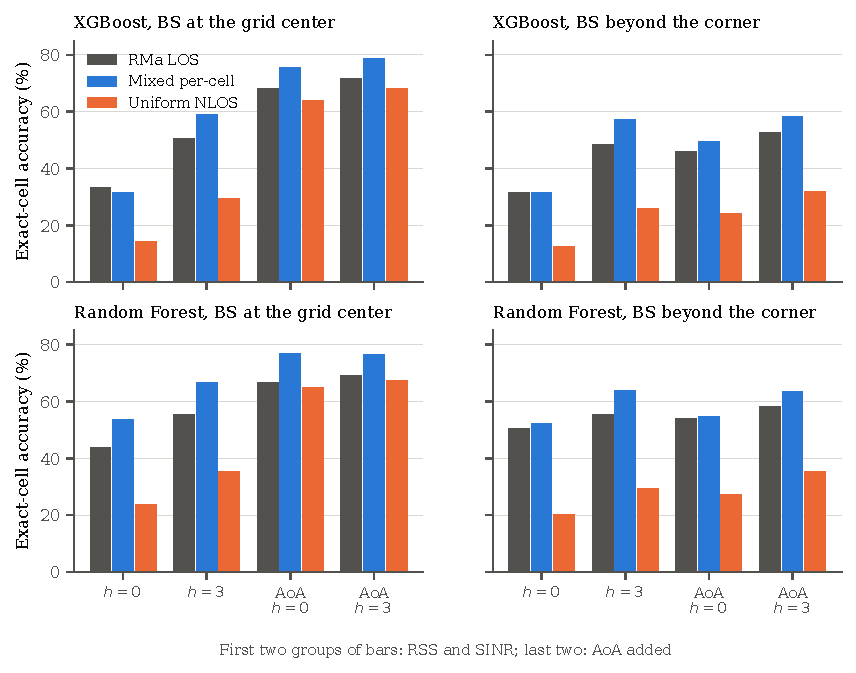
\includegraphics[width=0.82\textwidth]{fig_controlled_grid_sets}
  \captionof{figure}{Controlled grid: exact-cell accuracy at $h=0$ and $h=3$, from RSS and SINR and with AoA added, per classifier, BS placement and propagation setting. Single run per bar.}
  \label{fig:cg-sets}
\end{minipage}\par\medskip
% src: figure_scripts/python/make_figures_followup.py controlled_grid_sets(); comparison_sets.csv

\subsection{Macro-Cell Error Levels}
\label{app:macro-errors}

% src: naive_baseline/uniform_nlos (20 seeds: multi 35.27, single 38.50); pathloss_fit_summary.json (sigma_r 67.94 m at 95 m); seed_repeats_all_models_summary.json knn_h0 (23.38 / 46.17, five splits); followup_2026_10/uniform_nlos XGBoost snap / full (20 seeds: 18.74 / 15.59 multi, 36.33 / 36.51 single)
The constant guess, the ranging resolution of a single RSS reading, and the errors of the trained models are compared per device group in Table~\ref{tab:reference-levels}. A snapshot $k$-NN fingerprint, the classical approach, is worse than the constant guess for single-antenna devices, and the trained models remain about \SI{20}{\meter} apart between the two groups.

\par\medskip\noindent\begin{minipage}{\textwidth}
  \centering
  \captionof{table}{Macro cell, uniform NLOS: reference error levels per device group. The ranging resolution is a standard deviation, not an error.}
  \label{tab:reference-levels}
  \small
  \begin{tabular}{@{}lrr@{}}
    \toprule
    Reference & Multi-antenna & Single-antenna \\
    \midrule
    Constant guess~(mean training position, $20$ splits) & \SI{35.3}{\meter} & \SI{38.5}{\meter} \\
    RSS ranging resolution $\sigma_r$ at median range & \SI{68}{\meter} & \SI{68}{\meter} \\
    \midrule
    $k$-NN, $h=0$~(five splits) & \SI{23.4}{\meter} & \SI{46.2}{\meter} \\
    XGBoost, $h=0$~($20$ splits) & \SI{18.7}{\meter} & \SI{36.3}{\meter} \\
    XGBoost, $h=5$~($20$ splits) & \SI{15.6}{\meter} & \SI{36.5}{\meter} \\
    \bottomrule
  \end{tabular}
\end{minipage}\par\medskip

% src: diagnostics_2026_10/baseline_uniform_nlos/errors_first_seed.npz (seed 42); per_seed.xgboost.full (multi within 10 m 34 %, within 20 m 71 %, p50 13.7, p90 29.5; single 7 %, 21 %, 34.7, 59.1)
\par\medskip\noindent\begin{minipage}{\textwidth}
  \centering
  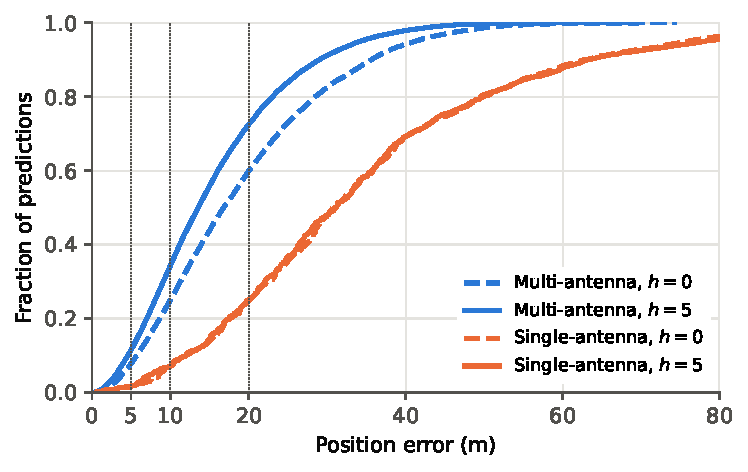
\includegraphics[width=0.65\textwidth]{fig_error_cdf}
  \captionof{figure}{Macro cell: distribution of position error per device group, XGBoost at $h=0$ and $h=5$, one split.}
  \label{fig:error-cdf}
\end{minipage}\par\medskip
% src: figure_scripts/python/make_figures_diagnostic.py error_cdf()
\par\medskip\noindent\begin{minipage}{\textwidth}
  \centering
  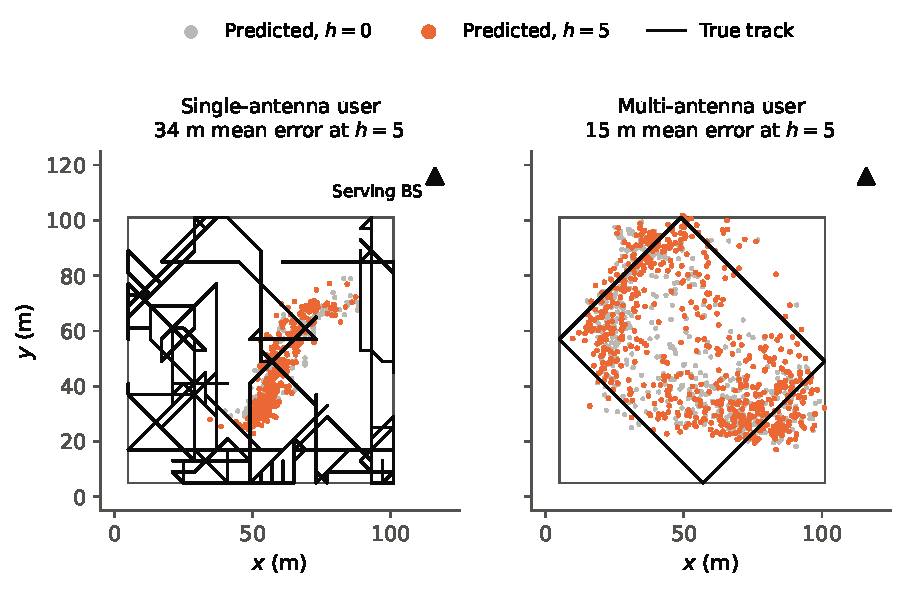
\includegraphics[width=0.75\textwidth]{fig_trajectories}
  \captionof{figure}{Macro cell: true track and predicted positions of the median single-antenna~(left) and multi-antenna~(right) test user, XGBoost at $h=0$ and $h=5$, one split.}
  \label{fig:trajectories}
\end{minipage}\par\medskip
% src: figure_scripts/python/make_figures_diagnostic.py trajectories(); diagnostics_2026_10/baseline_uniform_nlos/errors_first_seed.npz (seed 42; users 250 and 27)

\subsection{Per-Model History Gain in the Macro Cell}

Figure~\ref{fig:history-by-group} shows how the macro-cell gain builds with history depth, Table~\ref{tab:history-gain} gives the per-model values behind Figure~\ref{fig:history-gain-ci}, and Table~\ref{tab:supp-retune} gives the re-tuning check of Section~\ref{subsec:gain-macro}.

% src: history_sweep_all_models_summary.json curves (seed 42, multi_mae by depth); deep_history_sweep_trees_summary.json
\par\medskip\noindent\begin{minipage}{\textwidth}
  \centering
  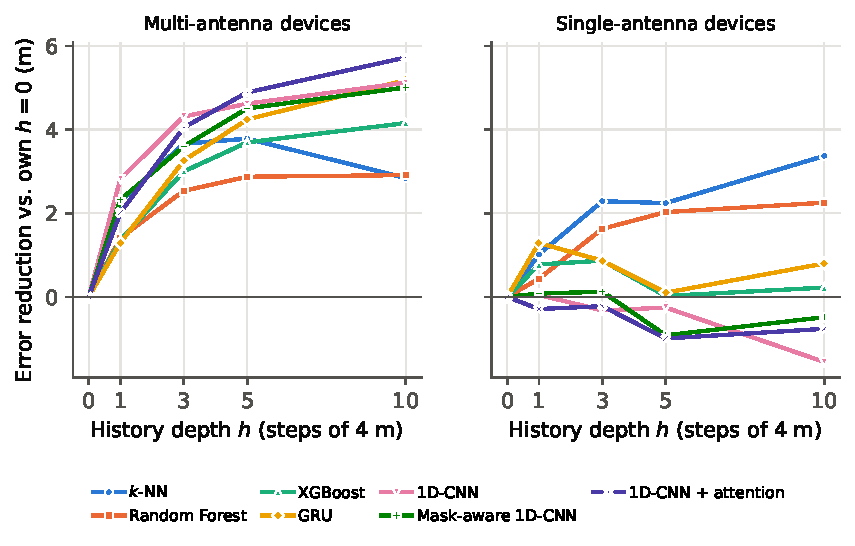
\includegraphics[width=0.85\textwidth]{fig_history_by_group}
  \captionof{figure}{Macro cell: error reduction against each model's own $h=0$ input as history depth grows, per device group, single split.}
  \label{fig:history-by-group}
\end{minipage}\par\medskip
% src: figure_scripts/python/make_figures.py history_by_group(); history_sweep_all_models_summary.json

\par\medskip\noindent\begin{minipage}{\textwidth}
  \centering
  \captionof{table}{Macro cell, uniform NLOS: error at $h=0$ and seed-paired gain from $h=0$ to $h=5$ per model and device group, with \SI{95}{\percent} Student-$t$ intervals, and cost of one run.}
  \label{tab:history-gain}
  \small
  \begin{tabular}{@{}lrrrrrr@{}}
    \toprule
     & \multicolumn{2}{c}{Multi-antenna devices} & \multicolumn{2}{c}{Single-antenna devices} & \multicolumn{2}{c}{Cost} \\
    \cmidrule(lr){2-3}\cmidrule(lr){4-5}\cmidrule(l){6-7}
    Model & Error, $h=0$ & Gain & Error, $h=0$ & Gain & Training & ms per 1000 \\
    \midrule
    $k$-NN & \SI{23.4}{\meter} & \SI{3.77 +- 0.47}{\meter} & \SI{46.2}{\meter} & \SI{-0.11 +- 3.28}{\meter} & \SI{1}{\second} & $577$ \\
    Random Forest$^\ast$ & \SI{18.8}{\meter} & \SI{2.75 +- 0.08}{\meter} & \SI{36.8}{\meter} & \SI{0.42 +- 0.39}{\meter} & \SI{34}{\second} & $102$ \\
    XGBoost$^\ast$ & \SI{18.7}{\meter} & \SI{3.15 +- 0.12}{\meter} & \SI{36.3}{\meter} & \SI{-0.18 +- 0.34}{\meter} & \SI{4}{\second} & $1.7$ \\
    GRU & \SI{19.3}{\meter} & \SI{3.54 +- 0.94}{\meter} & \SI{36.7}{\meter} & \SI{-0.26 +- 1.08}{\meter} & \SI{166}{\second} & $31$ \\
    1D-CNN & \SI{19.5}{\meter} & \SI{3.73 +- 1.20}{\meter} & \SI{36.0}{\meter} & \SI{-1.16 +- 2.59}{\meter} & \SI{197}{\second} & $14$ \\
    Mask-aware 1D-CNN & \SI{19.3}{\meter} & \SI{3.47 +- 1.06}{\meter} & \SI{34.8}{\meter} & \SI{0.25 +- 1.16}{\meter} & \SI{182}{\second} & $18$ \\
    1D-CNN + attention & \SI{19.5}{\meter} & \SI{4.06 +- 1.05}{\meter} & \SI{35.9}{\meter} & \SI{-1.39 +- 4.65}{\meter} & \SI{212}{\second} & $23$ \\
    \bottomrule
    \multicolumn{7}{@{}l}{\footnotesize $^\ast$~$20$ user splits; all other models five.}
  \end{tabular}
\end{minipage}\par\medskip
% src: errors and gains recomputed by figure_scripts/fig_history_gain_ci.m from data/seed_repeats_uniform_nlos.json (five splits) and data/followup20_uniform_nlos.json (20 splits; RF h=0 18.76 / 36.80, XGB 18.74 / 36.33); cost: master_benchmark_rerun_summary.json scorecard (train_time_sec, latency_ms_per_1k; k-NN cost row is the h=5 model)

\par\medskip\noindent\begin{minipage}{\textwidth}
  \centering
  \captionof{table}{Macro cell: overall mean error~(m) with fixed hyperparameters and with hyperparameters re-tuned at each depth on training users only, single split.}
  \label{tab:supp-retune}
  \small
  \begin{tabular}{@{}lrrrr@{}}
    \toprule
     & \multicolumn{2}{c}{XGBoost} & \multicolumn{2}{c}{Random Forest} \\
    \cmidrule(lr){2-3}\cmidrule(l){4-5}
    Depth & Fixed & Re-tuned & Fixed & Re-tuned \\
    \midrule
    $h=0$ & 22.35 & 21.91 & 22.11 & 22.05 \\
    $h=1$ & 21.12 & 21.20 & 20.91 & 20.84 \\
    $h=3$ & 19.80 & 19.66 & 19.77 & 19.81 \\
    $h=5$ & 19.43 & 19.07 & 19.42 & 19.40 \\
    $h=10$ & 19.03 & 18.97 & 19.34 & 19.30 \\
    \bottomrule
  \end{tabular}
\end{minipage}\par\medskip
% src: xgb_per_h_retune_summary.json, rf_per_h_retune_summary.json (as transcribed in FINAL_REPORT.md §5.5)

\subsection{Propagation and Interference}
\label{app:propagation}

% src: mixed_propagation_2026_09/pathloss_fit_summary.json zones.LOS (gamma 2.578, sigma 7.67 dB, R^2 0.261), zones.NLOS (gamma 3.595, sigma 11.89 dB, R^2 0.069); followup_2026_10/mixed_propagation/region_gain_did_vs_uniform.json (20 seeds: gap 1.81 +- 0.27 uniform, 1.54 +- 0.24 mixed; difference -0.27 +- 0.25; RF -0.01 +- 0.18)
In the mixed-propagation realization, a path-loss fit gives $\gamma = 2.58$ and a shadowing spread of \SI{7.7}{\decibel} in the LOS regions, against $\gamma = 3.60$ and \SI{11.9}{\decibel} in the NLOS regions. History lowers the multi-antenna error more in the LOS regions; however, the gap between the regions is the same in the uniform-NLOS realization of the same walks, which contains no LOS~(Figure~\ref{fig:los-nlos}), and its difference between the two realizations, \SI{-0.27 +- 0.25}{\meter} for XGBoost, is not distinguishable from zero. Table~\ref{tab:no-interference} gives the effect of removing the two interfering BSs.

\par\medskip\noindent\begin{minipage}{\textwidth}
  \centering
  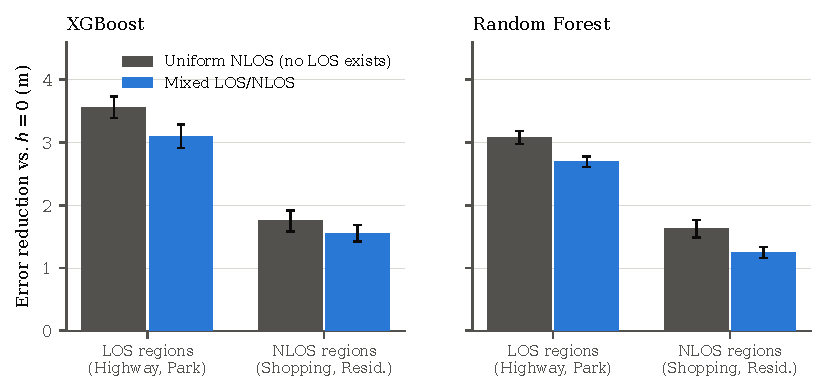
\includegraphics[width=0.8\textwidth]{fig_region_control}
  \captionof{figure}{Macro cell: reduction in multi-antenna error from history in the LOS and NLOS regions of the mixed realization and in the same regions of the uniform-NLOS realization. Seed-paired means over $20$ user splits with \SI{95}{\percent} Student-$t$ intervals.}
  \label{fig:los-nlos}
\end{minipage}\par\medskip
% src: figure_scripts/python/make_figures_followup.py region_control()

\par\medskip\noindent\begin{minipage}{\textwidth}
  \centering
  \captionof{table}{Macro cell: multi-antenna error at $h=0$ and gain from history, with and without the two interfering BSs, over $20$ user splits with \SI{95}{\percent} Student-$t$ intervals.}
  \label{tab:no-interference}
  \small
  \begin{tabular}{@{}llrrrr@{}}
    \toprule
    & & \multicolumn{2}{c}{Error at $h=0$} & \multicolumn{2}{c}{Gain from history} \\
    \cmidrule(lr){3-4}\cmidrule(l){5-6}
    Dataset & Model & with & without & with & without \\
    \midrule
    Uniform NLOS & XGBoost & $18.74$ & $19.30$ & $3.15 \pm 0.12$ & $3.44 \pm 0.17$ \\
    Uniform NLOS & Random Forest & $18.76$ & $19.34$ & $2.75 \pm 0.08$ & $3.15 \pm 0.11$ \\
    Mixed & XGBoost & $17.48$ & $18.46$ & $2.75 \pm 0.15$ & $3.15 \pm 0.17$ \\
    Mixed & Random Forest & $17.15$ & $18.14$ & $2.36 \pm 0.08$ & $2.80 \pm 0.09$ \\
    \bottomrule
  \end{tabular}
\end{minipage}\par\medskip
% src: followup_2026_10/no_interference/{uniform_nlos,mixed_propagation}/history_mechanism_followup_summary.json (20 seeds)


\end{document}
